% A LaTeX template for MSc Thesis submissions to 
% Politecnico di Milano (PoliMi) - School of Industrial and Information Engineering
%
% S. Bonetti, A. Gruttadauria, G. Mescolini, A. Zingaro
% e-mail: template-tesi-ingind@polimi.it
%
% Last Revision: October 2021
%
% Copyright 2021 Politecnico di Milano, Italy. NC-BY

\documentclass{Configuration_Files/PoliMi3i_thesis}

%------------------------------------------------------------------------------
%	REQUIRED PACKAGES AND  CONFIGURATIONS
%------------------------------------------------------------------------------

% CONFIGURATIONS
\usepackage{parskip} % For paragraph layout
\usepackage{setspace} % For using single or double spacing
\usepackage{emptypage} % To insert empty pages
\usepackage{multicol} % To write in multiple columns (executive summary)
\setlength\columnsep{15pt} % Column separation in executive summary
\setlength\parindent{0pt} % Indentation
\raggedbottom


% PACKAGES FOR TITLES
\usepackage{titlesec}
% \titlespacing{\section}{left spacing}{before spacing}{after spacing}
\titlespacing{\section}{0pt}{3.3ex}{2ex}
\titlespacing{\subsection}{0pt}{3.3ex}{1.65ex}
\titlespacing{\subsubsection}{0pt}{3.3ex}{1ex}
\usepackage{color}

% PACKAGES FOR LANGUAGE AND FONT
\usepackage[english]{babel} % The document is in English  
\usepackage[utf8]{inputenc} % UTF8 encoding
\usepackage[T1]{fontenc} % Font encoding
\usepackage[11pt]{moresize} % Big fonts

% PACKAGES FOR IMAGES
\usepackage{graphicx}
\usepackage{transparent} % Enables transparent images
\usepackage{eso-pic} % For the background picture on the title page
\usepackage{subfig} % Numbered and caption subfigures using \subfloat.
\usepackage{tikz} % A package for high-quality hand-made figures.
\usetikzlibrary{}
\graphicspath{{./Images/}} % Directory of the images
\usepackage{amsthm} % Coloured "Theorem"
\usepackage{thmtools}
\usepackage{xcolor}
\usepackage{float}

% STANDARD MATH PACKAGES
\usepackage{amsmath}
\usepackage{amssymb}
\usepackage{amsfonts}
\usepackage{bm}
\usepackage[overload]{empheq} % For braced-style systems of equations.
\usepackage{fix-cm} % To override original LaTeX restrictions on sizes

% PACKAGES FOR TABLES
\usepackage{tabularx}
\usepackage{longtable} % Tables that can span several pages
\usepackage{colortbl}

% PACKAGES FOR ALGORITHMS (PSEUDO-CODE)
\usepackage{algorithm}
\usepackage{algorithmic}

% PACKAGES FOR REFERENCES & BIBLIOGRAPHY
\usepackage[
    colorlinks=true,
    linkcolor=black,
    anchorcolor=black,
    citecolor=black,
    filecolor=black,
    menucolor=black,
    runcolor=black,
    urlcolor=black
]{hyperref} % Adds clickable links at references
\usepackage{cleveref}
\usepackage[square, numbers, sort&compress]{natbib} % Square brackets, citing references with numbers, citations sorted by appearance in the text and compressed
\bibliographystyle{abbrvnat} % You may use a different style adapted to your field

% OTHER PACKAGES
\usepackage{pdfpages} % To include a pdf file
\usepackage{afterpage}
\usepackage{lipsum} % DUMMY PACKAGE
\usepackage{fancyhdr}
\usepackage{wasysym} % For the headers
\usepackage{rotating}
\usepackage{listings}
%%
% Alloy language definition for using with the listings package.
%
% 2017, Daniel Andrade
% BSD 3-Clause License
%%
\lstdefinelanguage{alloy}{
    morekeywords={
        module, open, as,
        private, abstract, sig, extends, in,
        lone, some, one, disj,
        fact, pred, fun, assert,
        run, check,
        for, but, exactly,
        this, not, implies, else, let,
        not, no, set, all, sum,
        iff, or, Int, and,
        none, univ, iden
    },
    sensitive=true,
    morecomment=[l]{//},
    morecomment=[l]{--},
    morecomment=[s]{/*}{*/},
    morestring=[b]{"},
%literate={->}{$\rightarrow$}1
% replacing characters can cause problems when copying from PDF to editor
}[keywords,comments,strings]
\fancyhf{}

% Input of configuration file. Do not change config.tex file unless you really know what you are doing. 
% Define blue color typical of polimi
\definecolor{bluepoli}{cmyk}{0.4,0.1,0,0.4}

% Custom theorem environments
\declaretheoremstyle[
    headfont=\color{bluepoli}\normalfont\bfseries,
    bodyfont=\color{black}\normalfont\itshape,
]{colored}

% Set-up caption colors
\captionsetup[figure]{labelfont={color=bluepoli}} % Set colour of the captions
\captionsetup[table]{labelfont={color=bluepoli}} % Set colour of the captions
\captionsetup[algorithm]{labelfont={color=bluepoli}} % Set colour of the captions


\theoremstyle{colored}
\newtheorem{theorem}{Theorem}[chapter]
\newtheorem{proposition}{Proposition}[chapter]

% Enhances the features of the standard "table" and "tabular" environments.
\newcommand\T{\rule{0pt}{2.6ex}}
\newcommand\B{\rule[-1.2ex]{0pt}{0pt}}

% Pseudo-code algorithm descriptions.
\newcounter{algsubstate}
\renewcommand{\thealgsubstate}{\alph{algsubstate}}
\newenvironment{algsubstates}
{\setcounter{algsubstate}{0}%
\renewcommand{\STATE}{%
    \stepcounter{algsubstate}%
    \Statex {\small\thealgsubstate:}\space}}
{}

% New font size
\newcommand\numfontsize{\@setfontsize\Huge{200}{60}}

% Title format: chapter
\titleformat{\chapter}[hang]{
    \fontsize{50}{20}\selectfont\bfseries\filright}{\textcolor{bluepoli} \thechapter\hsp\hspace{2mm}\textcolor{bluepoli}{|   }\hsp}{0pt}{\huge\bfseries \textcolor{bluepoli}
}

% Title format: section
\titleformat{\section}
{\color{bluepoli}\normalfont\Large\bfseries}
{\color{bluepoli}\thesection.}{1em}{}

% Title format: subsection
\titleformat{\subsection}
{\color{bluepoli}\normalfont\large\bfseries}
{\color{bluepoli}\thesubsection.}{1em}{}

% Title format: subsubsection
\titleformat{\subsubsection}
{\color{bluepoli}\normalfont\large\bfseries}
{\color{bluepoli}\thesubsubsection.}{1em}{}

% Shortening for setting no horizontal-spacing
\newcommand{\hsp}{\hspace{0pt}}

\makeatletter
% Renewcommand: cleardoublepage including the background pic
\renewcommand*\cleardoublepage{%
    \clearpage\if@twoside\ifodd\c@page\else
    \null
    \AddToShipoutPicture*{\BackgroundPic}
    \thispagestyle{empty}%
    \newpage
    \if@twocolumn\hbox{}\newpage\fi\fi\fi}
\makeatother

%For correctly numbering algorithms
\numberwithin{algorithm}{chapter}

%----------------------------------------------------------------------------
%	NEW COMMANDS DEFINED
%----------------------------------------------------------------------------

%----------------------------------------------------------------------------
%	ADD YOUR PACKAGES (be careful of package interaction)
%----------------------------------------------------------------------------

%----------------------------------------------------------------------------
%	ADD YOUR DEFINITIONS AND COMMANDS (be careful of existing commands)
%----------------------------------------------------------------------------

\definecolor{dkgreen}{rgb}{0,0.6,0}
\definecolor{gray}{rgb}{0.5,0.5,0.5}
\definecolor{mauve}{rgb}{0.58,0,0.82}

\lstset{frame=tb,
    language=alloy,
    aboveskip=3mm,
    belowskip=3mm,
    showstringspaces=false,
    columns=flexible,
    basicstyle={\small\ttfamily},
    numbers=none,
    numberstyle=\tiny\color{gray},
    keywordstyle=\bf\color{blue},
    commentstyle=\it\color{dkgreen},
    stringstyle=\color{mauve},
    breaklines=true,
    breakatwhitespace=true,
    tabsize=3
}

%----------------------------------------------------------------------------
%	BEGIN OF YOUR DOCUMENT
%----------------------------------------------------------------------------

\begin{document}
    \fancypagestyle{plain}{%
        \fancyhf{} % Clear all header and footer fields
        \fancyhead[RO,RE]{\thepage} %RO=right odd, RE=right even
        \renewcommand{\headrulewidth}{0pt}
        \renewcommand{\footrulewidth}{0pt}}

%----------------------------------------------------------------------------
%	TITLE PAGE
%----------------------------------------------------------------------------

    \pagestyle{empty} % No page numbers
    \frontmatter % Use roman page numbering style (i, ii, iii, iv...) for the preamble pages

    \puttitle{
        title=Software Engineering 2\\Requirements Analysis and\\Specification Document
        \\[1cm] \textit{Students}\&\textit{Companies},
        name1=Belfiore Mattia,
        name2=Benedetti Gabriele,
        name3=Buccheri Giuseppe,
        academicyear=2024-2025
    }

%----------------------------------------------------------------------------
%	PREAMBLE PAGES: ABSTRACT (inglese e italiano), EXECUTIVE SUMMARY
%----------------------------------------------------------------------------
    \startpreamble
    \setcounter{page}{1} % Set page counter to 1

%----------------------------------------------------------------------------
%	LIST OF CONTENTS/FIGURES/TABLES/SYMBOLS
%----------------------------------------------------------------------------

% TABLE OF CONTENTS
    \thispagestyle{empty}
    \tableofcontents % Table of contents
    \thispagestyle{empty}
    \cleardoublepage

%-------------------------------------------------------------------------
%	THESIS MAIN TEXT
%-------------------------------------------------------------------------

    %\addtocontents{toc}{\vspace{2em}} % Add a gap in the Contents, for aesthetics
    \mainmatter % Begin numeric (1,2,3...) page numbering


    \chapter{Introduction}
    \label{ch:introduction}%
    In the real world, the process of finding suitable candidates for internships is often a complex and time-consuming task for companies, while university students face significant challenges in identifying opportunities that align with their skills, interests, and career aspirations. Companies have to consider numerous applications, many of which may not meet their requirements, and produce internship descriptions that attract the right talent. On the other hand, students are frequently left to navigate partial information sources, leading to inefficiencies and missed opportunities.
This disparity between the supply and demand for internships is caused by the lack of "ad hoc" tools to support efficient matchmaking. The success of an internship is often guaranteed by factors such as the relevance of candidates' skills to the offered projects, the clarity of internship descriptions, and the availability of resources like mentorship and training. Without a straight process, companies may struggle to identify candidates who fit their needs, and students may find it difficult to show their potential.
These challenges highlight the need for a unified platform that bridges the gap between students and companies, providing a mutually beneficial ecosystem where both parties can connect, evaluate, and collaborate. S\&C comes as a solution to address these pain points, offering a structured approach to simplifying and optimizing the internship process for all stakeholders involved.
\newpage

\section{Purpose}
\label{sec:purpose}%

\subsection{Goals}
\label{subsec:goals}%
\newcounter{g}
\setcounter{g}{1}
\newcommand{\cg}{\theg\stepcounter{g}}

Below there's a table that lists all the goals of the \verb|S&C| system:
\begin{center}
    \renewcommand{\arraystretch}{2}
    \begin{longtable}{ l p{0.8\linewidth} } 
        \hline
        \textbf{ID} & \textbf{Description}                                                                   \\
        \hline
        %%todo, mettere insieme 1-3 e 1-2
        G\cg  & Allows Companies to advertise their internship offers to find the most suitable students \\ \hline
        G\cg  & Allows Students to look for internships based on their needs \\ \hline
        G\cg  & Allows Students to be recommended to companies using keyword-based and statistical matching \\ \hline
        %%G\cg  & Allows Students to be notified when a new internship offer is published \\ \hline
        G\cg  & Supports selection process by helping manage interviews and also finalize the selections \\ \hline
        G\cg  & Provides suggestions to companies regarding how to make their offers more appealing for students \\ \hline
        G\cg  & Provides suggestions to students how to make their CVs more appealing for companies \\ \hline
        G\cg  & Allows stakeholders to monitor the progress of internships, report issues, and track outcomes \\ \hline
        G\cg  & Allows Universities to monitor the situation of ongoing internships and interrupt them when necessary \\ \hline
        \caption{The goals.}
        \label{tab:goals_tab}%
    \end{longtable}
\end{center}

\newpage


\section{Scope}
\label{sec:scope}%
The S\&C platform serves as a comprehensive system for matching students with internships and supporting related workflows. It acts as a hub for collaboration and interaction among three primary user groups: students, companies, and universities. Students are the primary user group, using the platform to create detailed profiles, upload and maintain updated CVs, search for internships manually, or receive personalized recommendations that better suit to their academic background, skills, and preferences. They can also apply to internships, participate in interviews with the help of the platform and finally provide feedback on their experiences, thereby contributing to the platform's constant improvement.
Companies utilize S\&C to manage their internship offerings and streamline recruitment. They can advertise internships with comprehensive descriptions, specifying required skills and qualifications, and benefit from a recommendation system that identifies suitable candidates. Companies can also review applications, shortlist applicants and schedule interviews within the platform. For the post-selection, they can provide feedback on students' performance, helping refine the matching algorithms and contributing to system insights.
Universities play a crucial supervisory role, ensuring the integrity and success of internships. They monitor ongoing internships, address complaints raised by students or companies and analyze trends to enhance their internship programs. Additionally, universities use the platform to ensure compliance with educational and legal standards, providing a secure and supportive environment for all parties involved.
Through the integration of these interactions, the S\&C platform simplifies the internship process while creating a cooperative environment that mutually supports students, companies, and universities.
\subsection{World phenomena}
\label{subsec:world_phenomena}%
\newcounter{wp}
\setcounter{wp}{1}
\newcommand{\cwp}{\thewp\stepcounter{wp}}
\begin{center}
    \renewcommand{\arraystretch}{2}
    \begin{longtable}{ l p{0.8\linewidth} } 
        \hline
        \textbf{ID} & \textbf{Description}                                                \\
        \hline
        WP\cwp      & A student wants to find an internship that meets his or her needs and goals\\
        \hline
        WP\cwp      & A student creates or update their CVs, reflecting their real-world skills and experiences   \\
        \hline
        WP\cwp      & A company decides to offer a new internship, defining its internship requirements and benefits \\
        \hline
        WP\cwp      & A student decides to accept or reject recommendations based on their preferences.          \\
        \hline
        WP\cwp      & A company decides to accept or reject recommendations based on their preferences                 \\
        \hline
        WP\cwp      & A company conducts interviews and evaluate candidates directly                   \\
        \hline
        WP\cwp      & Internships proceed in the real world, with students working on projects as described by the companies                                            \\
        \hline
        WP\cwp      & Stakeholders (students, companies, universities) identify issues during internships and report them to the appropriate parties.      \\
        \hline
        WP\cwp      & A university decides to interrupt an internship, based on the student or company complaints                       \\
        \hline
        \caption{World Phenomenas.}
        \label{tab:worldph_tab}%
    \end{longtable}
\end{center}

\subsection{Shared phenomena}
\label{subsec:shared_phenomena}%
\newcounter{sp}
\setcounter{sp}{1}
\newcommand{\csp} {\thesp\stepcounter{sp}}
\begin{center}
\renewcommand{\arraystretch}{2}

\paragraph{Shared Phenomena - World Controlled}

\begin{longtable}{ l p{0.8\linewidth} }
    \hline
    \textbf{ID} & \textbf{Description} \\ 
    \hline
    SP\csp & A student signs up to the system or logs in if already registered, using the academic email address \\ 
    \hline
    SP\csp & A company signs up to the system or logs in if already registered \\ 
    \hline
    SP\csp & A student uploads his CV \\ 
    \hline
    SP\csp & A student uploads additional personal information to guarantee better matching \\ 
    \hline
    SP\csp & A student chooses to accept a recommended internship \\ 
    \hline
    SP\csp & A student provides feedback and suggestions on how to improve a recently completed internship \\ 
    \hline
    SP\csp & A student provides problems or complaints about an ongoing internship \\ 
    \hline
    SP\csp & A company provides additional information to guarantee better matching \\ 
    \hline
    SP\csp & A company publishes and manages internship offers through the system interface \\ 
    \hline
    SP\csp & A company chooses to accept a recommended student for a specific internship \\ 
    \hline
    \caption{Shared Phenomena - World Controlled.}
    \label{tab:sharedph_world_tab}%
\end{longtable}

\paragraph{Shared Phenomena - Machine Controlled}

\begin{longtable}{ l p{0.8\linewidth} }
    \hline
    \textbf{ID} & \textbf{Description} \\ 
    \hline
    SP\csp & The system provides personalized recommendations for internships to a student \\ 
    \hline
    SP\csp & The system provides personalized recommendations for candidates to a company \\ 
    \hline
    SP\csp & The system supports companies by organizing interviews and collecting structured questionnaire responses \\ 
    \hline
    SP\csp & The system offers personalized suggestions for improving CV to a student \\ 
    \hline
    SP\csp & The system offers personalized suggestions for improving job postings to a company \\ 
    \hline 
    SP\csp & The system sends a notification to a student of a new internship offer that meets his needs \\ 
    \hline 
    SP\csp & The system enables users to submit and manage complaints, facilitating resolution with relevant stakeholders. \\ 
    \hline
    \caption{Shared Phenomena - Machine Controlled.}
    \label{tab:sharedph_machine_tab}%
\end{longtable}

\end{center}

\section{Definition, Acronyms, Abbreviations}
\label{sec:definition_acronyms_abbreviations}%
\begin{table}[H]
    \begin{center}
        \begin{tabular}{ |l|l| }
            \hline
            \textbf{Acronyms} & \textbf{Definition}                              \\
            \hline
            RASD & Requirements Analysis and Specification Document \\ \hline
            S\&C & Students\&Companies \\ \hline
            CV & Curriculum Vitae \\ \hline
        \end{tabular}
        \caption{Acronyms used in the document.}
        \label{tab:acronyms}%
    \end{center}
\end{table}


\section{Revision history}
\label{sec:revision_history}%
 \begin{itemize}
     \item Version 1.0 - 22/12/2024
 \end{itemize}

\section{Reference Documents}
\label{sec:reference_documents}%
\begin{itemize}
    \item Assignment document
    \item CreatingRASD (lecture slides)
\end{itemize}


\section{Document Structure}
\label{sec:document_structure}%
\begin{itemize}
    \item \textbf{Introduction}: A general introduction to the goals, the phenomena and the scope of
            the system. It provides general but exhaustive information about what the RASD
            document is going to explain.
    \item \textbf{Overall Description}: A general description of the product to be,its requirements and the scenarios that might occur.
    \item \textbf{Specific Requirements:} All software requirements are explained using scenarios,
            use-case diagrams and activity diagrams. It focuses on the specific requirements and provides a more
            detailed analysis of external interface requirements, functional requirements and performance ones.
    \item \textbf{Formal Analysis Using Alloy:} This section includes Alloy code that describes the
            model and shows its soundness and correctness.
    \item \textbf{Effort Spent:} Effort spent by all team members shown as the list of all the activities
            done during the realization of this document
    \item \textbf{References:} References to documents that this project was developed upon.
\end{itemize}



    \chapter{Overall Description}
    \label{ch:overall_description}%
    \section{Product perspective}
\label{sec:product_perspective}%



\subsection{Scenarios}
\label{subsec:scenarios}%
\begin{itemize}
    \item \textbf{Scenario 1 : Companies Submit Internship Postings}

Companies create and publish detailed internship descriptions, specifying roles, qualifications, benefits, and deadlines. They ensure that the postings are tailored to attract the right candidates. Companies can also update these postings to reflect changes or clarify details as needed, ensuring that they remain appealing and informative.
    \item \textbf{Scenario 2 : Students Create Profiles and Upload CVs}

Students register on the platform and complete their profiles by entering academic background, skills, extracurricular activities, and personal preferences for internships. They upload polished and revised CVs that highlight their qualifications, ensuring visibility to potential employers. The platform may also provide guidance on enhancing CV quality to improve students' chances of selection. 
    \item \textbf{Scenario 3 : Students Browse and Apply for Internships} 

Students actively explore the internship database on the platform using filters such as preferred location, required skills, and duration. The system allows students to compare internships and apply to multiple opportunities at the same time, making the application process efficient and maximizing their chances of success.
    \item \textbf{Scenario 4 : \textbf{System Recommends Internships to Students} }

Using advanced matching algorithms, the platform suggests internships that align with the profile, academic qualifications and career goals of the student. These recommendations adapt over time based on student interactions, applications and feedback, creating a highly personalized experience.
\item \textbf{Scenario 5 : \textbf{Companies Receive and Review Applications} }

Companies access a dashboard dedicated to them in order to view applications submitted by students. They evaluate candidates by comparing their profiles and CVs with internship requirements. The platform provides tools to rank applicants, add notes, and collaboratively review candidates with team members.
\item \textbf{Scenario 6 :\textbf{Interview Scheduling and Management}}

The platform simplifies interview logistics by giving companies the opportunity to schedule interviews with selected candidates. Supporting virtual meeting integrations and sending automated reminders to ensure all parties are prepared. The system also tracks the results of the interviews for later reference.
\item \textbf{Scenario 7 : Feedback Collection:} 

Both students and companies submit structured feedback after each major milestone, such as application reviews or interviews. This feedback is used to refine the profiles of students, improve internship postings, and enhance the platform’s recommendation capabilities. Feedback mechanisms also promote transparency and accountability.
\item \textbf{Scenario 8 : \textbf{Internship Monitoring by Universities} }

Universities oversee active internships by receiving updates on student performance, company satisfaction, and project progress. They use dashboards to track multiple internships simultaneously and ensure compliance with educational objectives. Universities can also intervene when problems are reported.
\item \textbf{Scenario 9 : \textbf{Complaint Handling}}

An efficiently working complaint management system allows students and companies to raise concerns during internships. Complaints are directed to universities that investigate and mediate to resolve conflicts. The system records the entire process to ensure fairness and transparency.
\item \textbf{Scenario 10 : \textbf{System Updates Recommendations} }

The platform’s recommendation engine evolves based on user feedback, application trends, and internship results. This dynamic update feature ensures future recommendations are more accurate and relevant, helping both students and companies.
\item \textbf{Scenario 11 : \textbf{Post-Internship Evaluation} }

After completing internships, students and companies provide detailed evaluations of their experiences. These evaluations highlight strengths, areas for improvement, and contribute to building a database of internship performance indicators for future users.
\item \textbf{Scenario 12 : Statistical Data Analysis} 

The platform collects data on applications, student performance, and company satisfaction. Advanced statistical tools analyze these data to uncover trends such as popular skills, successful industries, or common challenges. Insights from these analyses inform strategic improvements.
\item \textbf{Scenario 13 : Notifications and Alerts} 

The platform ensures that users are continuously informed through real-time notifications. Students receive alerts about new internships that match their profiles, upcoming deadlines, or interview schedules. Companies are notified of new applications, interview confirmations, and feedback submissions, ensuring timely responses and actions.
\end{itemize}
\subsection{Class Diagrams}
\label{subsec:class_diagrams}%
\begin{figure}[H]
    \centering
    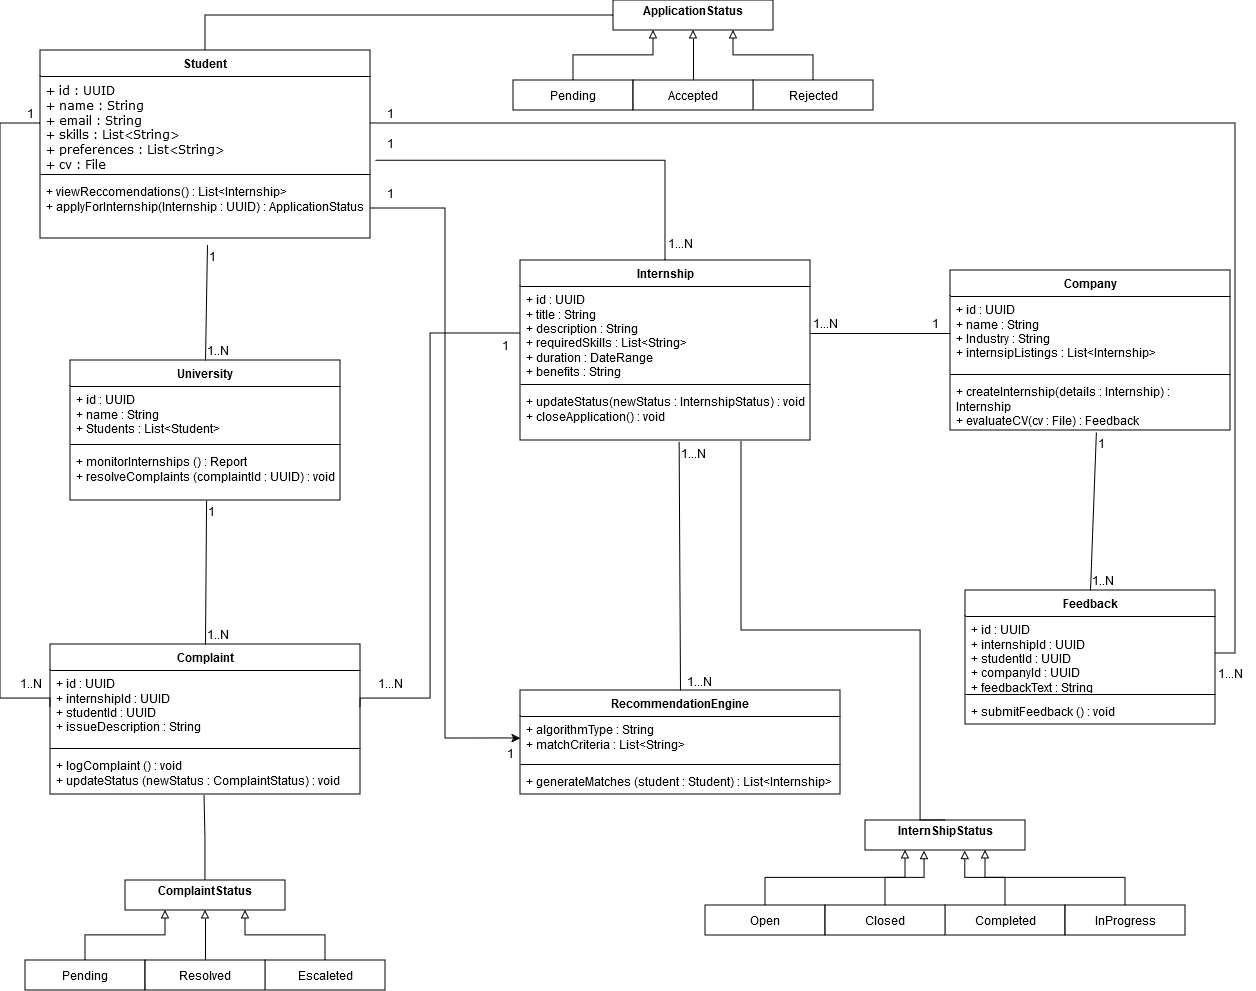
\includegraphics[width=1\linewidth]{Images/Class diagrams/ClassDiagram.png}
    \caption{Class Diagram}
    \label{fig:enter-label}
    
    
\end{figure}

\subsection{State Diagrams}
\label{subsec:class_diagrams}%

\paragraph{Sign-up} Initially, users can create a generic account that allows them to browse available posts without the ability to post. To upgrade to a full account, they must verify their email address, select a role (either as a student or a company), and complete the required fields for their chosen role.

\begin{figure}[H]
    \centering
    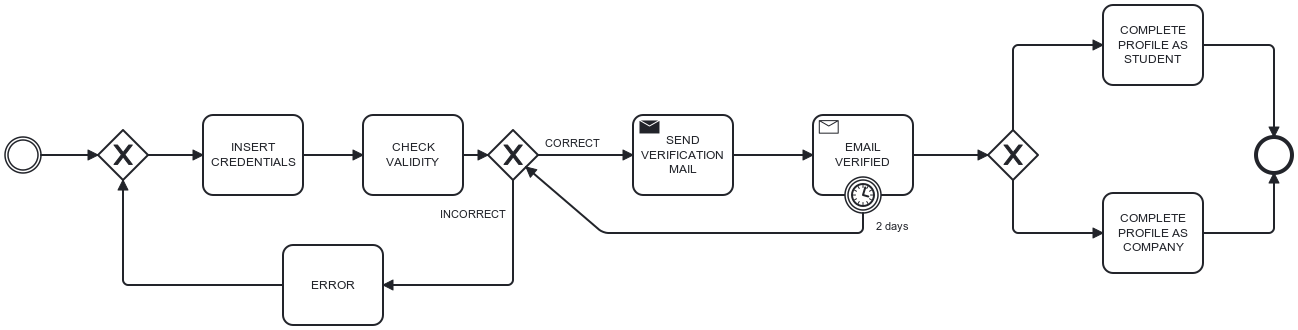
\includegraphics[width=1\linewidth]{Images//state diagrams/SIGNUP.png}
    \caption{Sign-up state diagram}
    \label{fig:enter-label}
\end{figure}

\paragraph{Login} During login, the system verifies the user's credentials to ensure they are correct. Upon successful authentication, the user is redirected to their personalized homepage.

\begin{figure}[H]
    \centering
    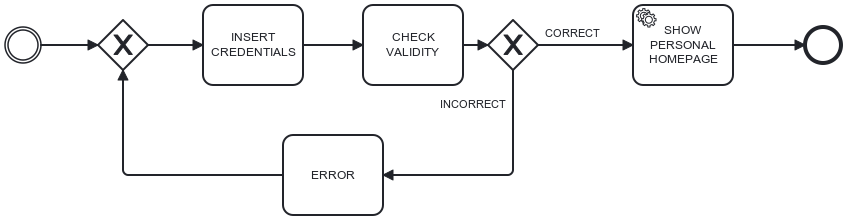
\includegraphics[width=1\linewidth]{Images//state diagrams/LOGIN.png}
    \caption{Login state diagram}
    \label{fig:enter-label}
\end{figure}

\paragraph{Apply for an internship} The student reviews their recommended internships. If they decide to apply for one, they must contact the company, which will proceed to schedule an interview. If the interview is successful and both parties agree, the internship will be communicated to the university.

\begin{figure}[H]
    \centering
    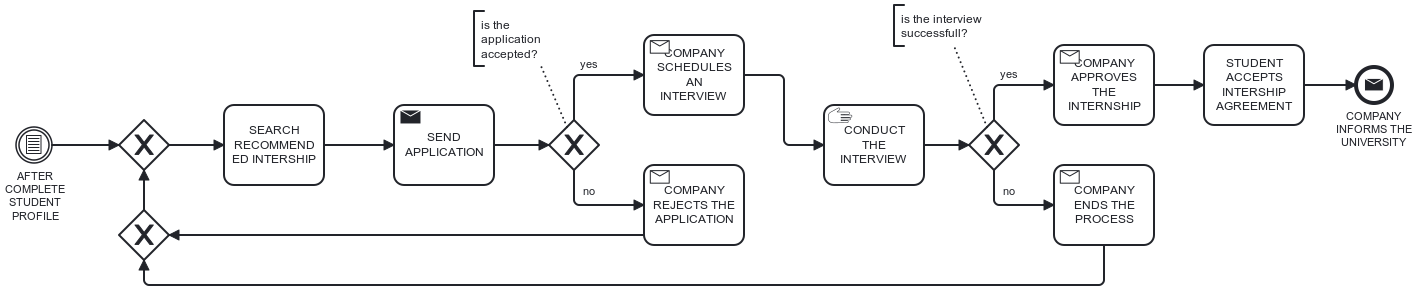
\includegraphics[width=1\linewidth]{Images//state diagrams/APPLICATION.png}
    \caption{Application state diagram}
    \label{fig:enter-label}
\end{figure}

\paragraph{Complaints handling} Both students and companies can submit a complaint during the internship. The university evaluates the complaint to determine whether intervention is necessary. If no intervention is required, the process ends without further action. However, if intervention is necessary, the university attempts to mediate between the parties to resolve the issue. If mediation is successful, the process concludes, and the internship continues as usual. On the other hand, if mediation fails or the issue remains unresolved, the university decides to terminate the internship. Before finalizing the termination, the university ensures that both parties are informed about the decision.

\begin{figure}[H]
    \centering
    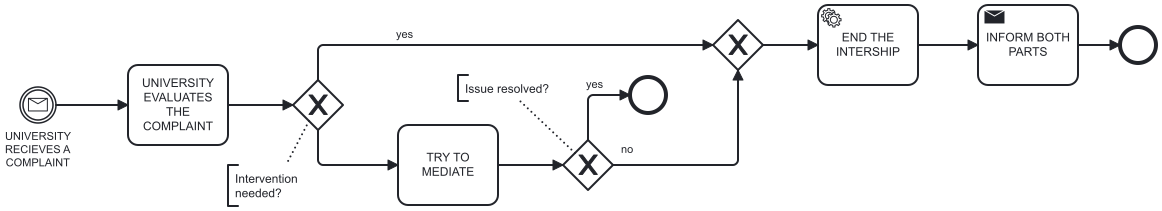
\includegraphics[width=1\linewidth]{Images//state diagrams/COMPLAINTS.png}
    \caption{Complaint diagram}
    \label{fig:enter-label}
\end{figure}

\section{Product functions}
\label{sec:product_functions}%

Here's the main functions of S\&C system:

\paragraph{Register to the platform}
The S\&C platform allows students and companies to register. During the registration process, users are required to provide the following information:
\begin{center}
\renewcommand{\arraystretch}{1}
\begin{tabular}{|p{5cm}|p{5cm}|p{5cm}|}
\hline
\textbf{Field} & \textbf{Required for} & \textbf{Notes} \\
\hline
Role & Both & Student or Company \\
\hline
Full name & Both &  \\
\hline
Company name & Company only &  \\
\hline
Email address & Both & Checking valid email address \\
\hline
Password & Both & Checking security standards \\
\hline
Attending university & Student only & Checking an existing university name \\
\hline
Phone number & Both &  \\
\hline
Postal Code & Both & Matching parameter \\
\hline
Office address & Company only & Matching parameter \\
\hline
Office phone number & Company only & Optional \\
\hline
\end{tabular}
\end{center}

While registering to the system, users must first declare that they have read and understood the Privacy Statement. They are also required to accept the Terms and Conditions, which request consent for the acquisition and processing of their personal data for the purpose of using the platform's matching analysis.

\paragraph{Post an internship}A button within the company's dashboard that opens a form for creating and submitting a new internship posting, including fields for job title, description, requirements, salary, and duration

\paragraph{Check recommended internships}A searchable and filterable page accessible to all users, displaying a list of internships with brief descriptions and company details.
\paragraph{Apply for an internship}A button on each internship's detail page that triggers a form submission, allowing students to send their application with a personalized message and resume upload.
\paragraph{Evaluate an application}A company dashboard feature showing a list of received applications with applicant details, resumes, and the option to accept, reject, or schedule interviews.
\paragraph{Schedule an interview}An action available on an application detail page that opens a scheduling form, allowing the company to set the interview's date, time, and mode.
\paragraph{Submit a complaint}A button in the dashboard (available to students and companies) that opens a form for submitting a formal complaint, including issue details.
\paragraph{Submit a feedback}A post-internship form accessible to both students and companies where they can rate the experience, provide comments, and suggest improvements for future internships.

\section{User characteristics}
\label{sec:user_characteristics}%

The actors of the application are the following:

\begin{itemize}
    \item \textbf{Student}: A single person registered as a student on the platform. Their aim is to find internships aligned with their academic background, skills, and career goals. They need only an active account, an internet connection, and access to a digital CV.
    \item \textbf{Company}: An organization of people registered on the platform. Its goal is to publish internship opportunities, examine applications, and hire suitable candidates. It requires an active account, an internet connection, and major internship details.
    \item \textbf{University}: A career services representative with a passive role on the platform. Universities are contacted only if an internship goes wrong or complaints emerge from companies or students. Their task is to review the situation and, if necessary, interrupt the internship. They need access to relevant student and company data.
\end{itemize}

\section{Assumptions, dependencies and constraints}
\label{sec:assumptions_dependencies_and_constraints}%
\newcounter{da} 
\setcounter{da}{1}
\newcommand{\cda}{D\arabic{da}\stepcounter{da}} 
\begin{center}
    \renewcommand{\arraystretch}{2}
    \begin{longtable}{ l p{0.8\linewidth} } 
        \hline
        \textbf{ID} & \textbf{Description} \\ 
        \hline
        \cda & Internship descriptions are comprehensive and reliable \\ \hline
        \cda & CVs accurately reflect students' skills and experiences \\ \hline
        \cda & Universities actively oversee internships and intervene when necessary \\ \hline
        \cda & Companies manage interview timelines and conduct them professionally \\ \hline
        \cda & Users provide meaningful feedback to improve the system \\ \hline
        \cda & Problems are reported in a timely manner by all parties \\ \hline
        \cda & The platform supports high user traffic without performance issues \\ \hline
        \caption{Domain Assumptions.}
        \label{tab:worldph_tab}%
    \end{longtable}
\end{center}




    \chapter{Specific Requirements}
    \label{ch:specific_requirements}%
    \section{External Interface Requirements}
\label{sec:external_interface_requirements}%

\subsection{User Interfaces}
\label{subsec:user_interfaces}%
The platform will provide have different interfaces for each one of its three primary user groups: students, companies, and universities. Each interface will be role-specific in order to facilitate interactions. The student interface will include a dashboard summarizing recommended internships, application statuses, and interview schedules; there will be also a profile editor for updating academic details, skills, and preferences; every student will be provided a search interface with filters (e.g., location, skills, duration) to browse available internships. The company interface will feature tools to create, edit, and manage internship postings; a dashboard to view applications, candidates lists  and scheduled interviews. The university interface will instead include a dashboard displaying active internships, student feedback and complaint statuses; the university interface is equipped with tools to analyze trends and generate reports on internship outcomes as well as a complaint resolution module to address issues raised by students or companies.

\subsection{Hardware Interfaces}
\label{subsec:hardware_interfaces}%
The platform is a web app; this means that it does not require any specific hardware interface except for a computer or any other device with web browser.  
\subsection{Software Interfaces}
\label{subsec:software_interfaces}%
In order to work correctly, the system will need to integrate with a few software components; here they are listed in detail:
\begin{itemize}
    \item \textbf{Database Systems:} To store user profiles, internship details, application records, and feedback securely.
    \item \textbf{Email and Notification APIs:} To send updates and reminders to users about critical events such as deadlines or feedback.
    \item \textbf{Video Conferencing Tools:} For virtual interviews between students and companies.
    \item \textbf{Statistical Analysis Tools:} To extract meaningful data from user interactions and feedback.
\end{itemize}
 
\subsection{Communication Interfaces}
\label{subsec:communication_interfaces}%
The platform will support secure communication protocols to facilitate data exchange and guarantee privacy.  The user will use internet access to access the platform and use the functionalities, such as logging in, contacting other users and reporting feedback on interviews or students. The platform must be HTTPS compliant in order to work on the web properly and to be safe. 
 
\section{Functional Requirements}
\label{sec:functional_requirements}%

\subsection{Requirements}
\label{subsec: requirements}%
\newcounter{h}
\setcounter{h}{0}
\newcommand{\ch}{\stepcounter{h}R\theh}

\begin{center}
    \renewcommand{\arraystretch}{2}
    \begin{longtable}{ l p{0.8\linewidth} } 
        \hline

        \textbf{ID} & \textbf{Description}                                                \\
        \hline
        \ch      & S\&C system allows unregistered users to sign-up.\\
        \hline
        \ch      & S\&C system allows registered users to verify their email address.\\
        \hline
        \ch      & S\&C system allows registered users to login.   \\
        \hline
        \ch      & S\&C system allows registered users to edit their account details.   \\
        \hline
        \ch      & S\&C system allows registered users to delete their account.   \\
        \hline
        \ch      & S\&C system allows registered users to view posted internships on the platform.   \\
        \hline
        \ch      & S\&C system allows registered users to upgrade to a Student account or a Company account. \\                     
        \hline
        \ch      & S\&C system allows registered users to verify their current academic status by validating their institutional email address.\\                     
        \hline
        \ch      & S\&C system allows registered users to update their notifications preferences.\\
        \hline
        \ch      & S\&C system allows Students to view a personalized dashboard in their homepage.\\  
        \hline
        \ch      & S\&C system allows Students to explore available internships. \\  
        \hline
        \ch      & S\&C system allows Students to view available internships ordered by the best matching, based on a matching score system. \\
        \hline
        \ch      & S\&C system allows Students to change the default order. \\
        \hline
        \ch      & S\&C system allows Students to apply filters on the view of the available internships. \\
        \hline
        \ch      & S\&C system allows Students to receive notification when a new internship matching their profile is posted.\\  
        \hline
        \ch      & S\&C system allows Students to view the details of a specific internship page. \\ 
        \hline
        \ch      & S\&C system allows Students to apply for an internship.\\ 
        \hline
        \ch      & S\&C system allows Students to view sent applications.\\ 
        \hline
        \ch      & S\&C system allows Students to monitor the status of an application.\\ 
        \hline
        \ch      & S\&C system allows Students to withdraw a sent application.\\ 
        \hline
        \ch      & S\&C system allows Students to confirm their participation of a scheduled interview via a notification interface.\\
        \hline
        \ch      & S\&C system allows Students to decline an interview offer via a notification interface.\\
        \hline
        \ch      & S\&C system sends automated reminders to Students for upcoming interview deadlines.\\
        \hline
        \ch      & S\&C system allows Students to review the agreements of an internship before accepting.\\ 
        \hline
        \ch      & S\&C system allows Students to file a complaint. \\ 
        \hline
        \ch      & S\&C system allows Students to submit feedback after completing an internship.\\ 
        \hline
        \ch      & S\&C system allows Companies to post internship offers by providing detailed information\\ 
        \hline
        \ch      & S\&C system allows Companies to edit an internship's post. \\  
        \hline
        \ch      & S\&C system allows Companies to delete an internship's post. \\  
        \hline
        \ch      & S\&C system allows Companies to identify the most suitable students on the platform for their internship posts, even if the students have not applied.\\
        \hline
        \ch      & S\&C system allows Companies to review the applications for an internship. \\
        \hline
        \ch      & S\&C system allows Companies to view internship's applications ordered by the best match. \\
        \hline
        \ch      & S\&C system allows Companies to receive notification when a new students with an high matching score has applied.\\  
        \hline
        \ch      & S\&C system allows Companies to propose a date to a student to schedule an interview. \\  
        \hline
        \ch      & S\&C system allows Companies to prepare a standardized set of questions to be proposed to all candidates for a specific internship.\\  
        \hline
        \ch      & S\&C system allows Companies compare the answers from all candidates to facilitate the selection process.\\  
        \hline
        \ch      & S\&C system allows Companies to reject a students after the interview. \\
        \hline
        \ch      & S\&C system allows Companies to start an internship. \\  
        \hline
        \ch      & S\&C system allows Companies to view active internships. \\
        \hline
        \ch      & S\&C system allows Companies to file a complaint.\\ 
        \hline
        \ch      & S\&C system allows Companies to submit feedback after completing an internship.\\ 
        \hline
        \ch      & S\&C system allows universities to login to the system providing credentials.\\ 
        \hline
        \ch      & S\&C system allows universities to collect complaints raised by Students.\\ 
        \hline
        \ch      & S\&C system allows universities to collect complaints raised by Companies.\\ 
        \hline
        \ch      & S\&C system allows universities to mediate between Student and Company after a complaint.\\ 
        \hline
        \ch      & S\&C system improves recommendation accuracy by considering user feedback on previous internships.\\ 
        \hline
        \ch      & S\&C system periodically updates internship recommendations based on new data from Students and Companies.\\ 
        \hline
        \caption{Requirements}
        \label{tab:worldph_tab}%
    \end{longtable}
\end{center}

\subsection{Use case diagrams}
\label{subsec: use_case_diag}%

\begin{figure}[H]
    \centering
    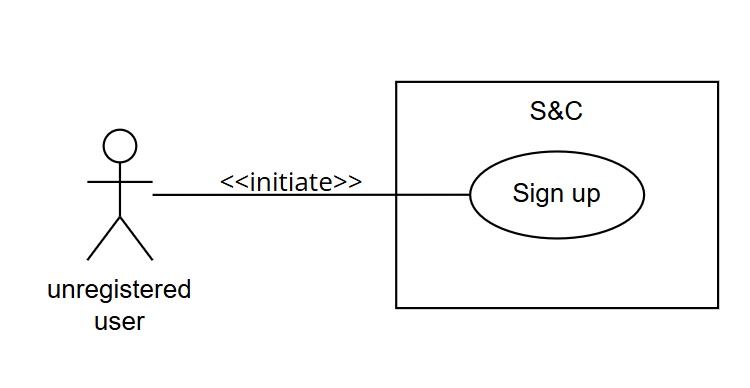
\includegraphics[width=1\linewidth]{Images/use case diagrams/UNREGISTERED_USER.png}
    \caption{Unregistered user use case diagram}
    \label{fig:enter-label}
\end{figure}

\begin{figure}[H]
    \centering
    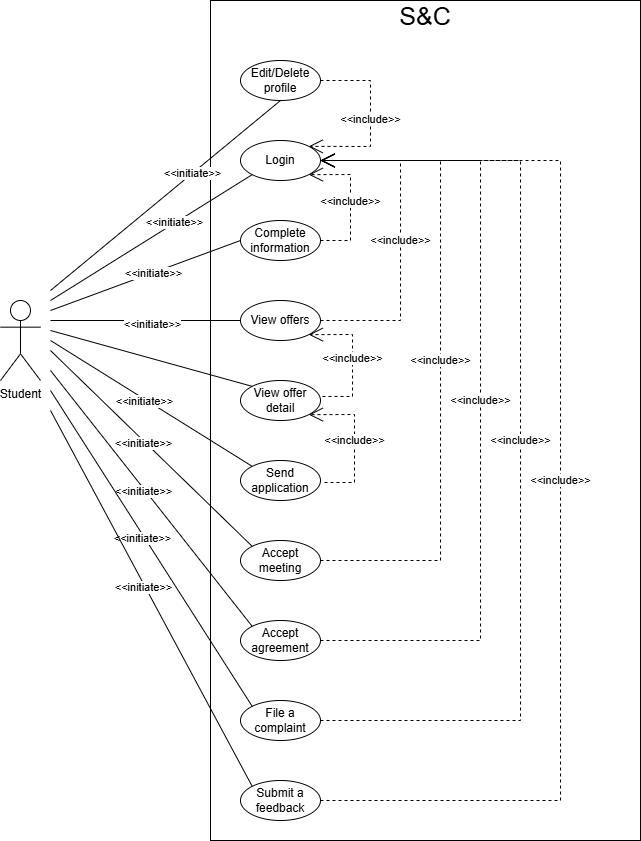
\includegraphics[width=1\linewidth]{Images/use case diagrams/STUDENT.png}
    \caption{Student use case diagram}
    \label{fig:enter-label}
\end{figure}

\begin{figure}[H]
    \centering
    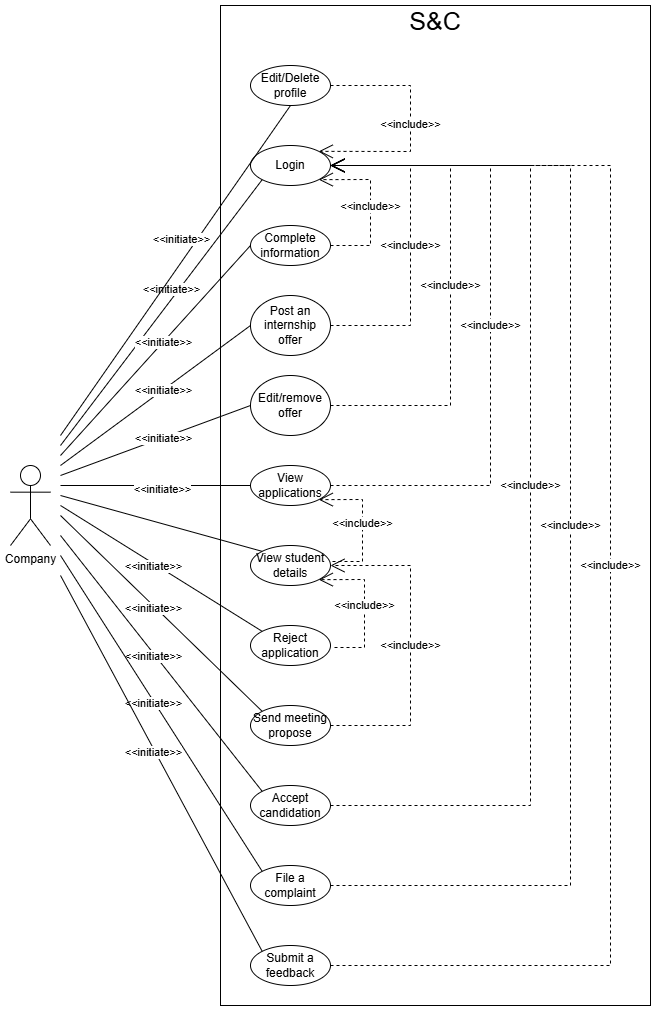
\includegraphics[width=0.9\linewidth]{Images/use case diagrams/COMPANY.png}
    \caption{Company use case diagram}
    \label{fig:enter-label}
\end{figure}

\begin{figure}[H]
    \centering
    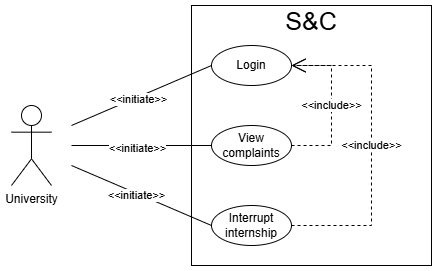
\includegraphics[width=1\linewidth]{Images/use case diagrams/UNIVERSITY.png}
    \caption{University use case diagram}
    \label{fig:enter-label}
\end{figure}

\subsection{Use cases}
\label{subsec: use_cases}%

\newcounter{uc}
\setcounter{uc}{1}
\newcommand{\cuc}{\theuc\stepcounter{uc}}

\textbf{UC\cuc\  - User registration}

\begin{center} 
    \renewcommand{\arraystretch}{1.2} 
    \begin{longtable}{ l p{0.8\linewidth} } 
        \hline 
        Actor & Unregistered User \\ \hline 
        Entry Condition & The user does not have an account and clicks the "Sign Up" button to create a new one. \\ \hline 
        Event Flow & 1.\ The unregistered user opens the S\&C application and clicks the "Sign Up" button. \\ 
        & 2.\ The user fills out all mandatory fields (email, password) and confirms the password. \\ 
        & 3.\ The user agrees to the "Terms \& Conditions" and "Privacy Policy" by checking the corresponding boxes. \\ 
        & 4.\ The user presses the "Sign Up" button to submit the registration form. \\ 
        & 5.\ The S\&C system sends a confirmation email to the provided email address. \\ 
        & 6.\ The user completes the registration by clicking the confirmation link in the email. \\ \hline 
        Exit Condition & The user's account is successfully created, and they can log into the system. \\ \hline 
        Exceptions & 1.\ One or more mandatory fields are empty. \\ 
        & 2.\ An account with the same email already exists. \\ 
        & 3.\ The user has not checked the "Terms \& Conditions" or "Privacy Policy" boxes. \\ \hline 
        \caption{Unregistered User registration process} 
        \label{tab:user_registration_uc} 
    \end{longtable} 
\end{center}

\begin{figure}[H]
    \centering
    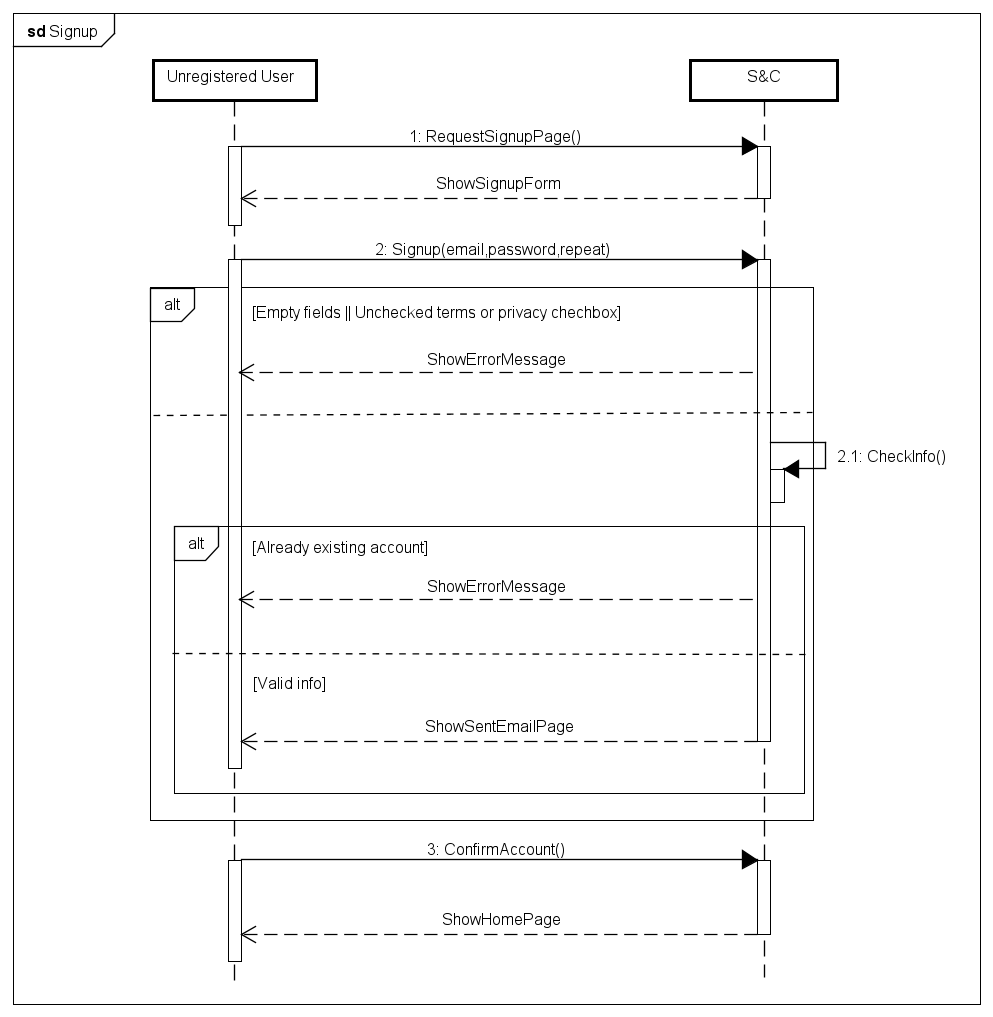
\includegraphics[width=1\linewidth]{Images/Sequence diagrams/Signup.png}
    \caption{User registration sequence diagram}
    \label{fig:enter-label}
\end{figure}

\textbf{UC\cuc\  - User, student, company or university login}

\begin{center}
    \renewcommand{\arraystretch}{1.2} 
    \begin{longtable}{ l p{0.8\linewidth} } 
        \hline
        Actor & Registered user (student, company, or university). \\ \hline
        Entry Condition & A user with an existing account clicks the "Login" button to access the homepage of the S\&C platform. \\ \hline
        Event Flow & 1.\ The user enters their credentials (email, password) in the login form. \\ 
        & 2.\ The user presses the "Login" button. \\ 
        & 3.\ The S\&C system validates the provided credentials. \\ \hline
        Exit Condition & If the credentials are correct, the user is redirected to the homepage. \\ \hline
        Exceptions & 1.\ The provided email is not registered in the platform. \\ 
        & 2.\ The provided password is incorrect. \\ 
        & 3.\ One or both fields (email or password) are left empty. \\ \hline
        \caption{Registered user logs in.}
        \label{tab:goals_tab}%
    \end{longtable}
\end{center}


\begin{figure}[H]
    \centering
    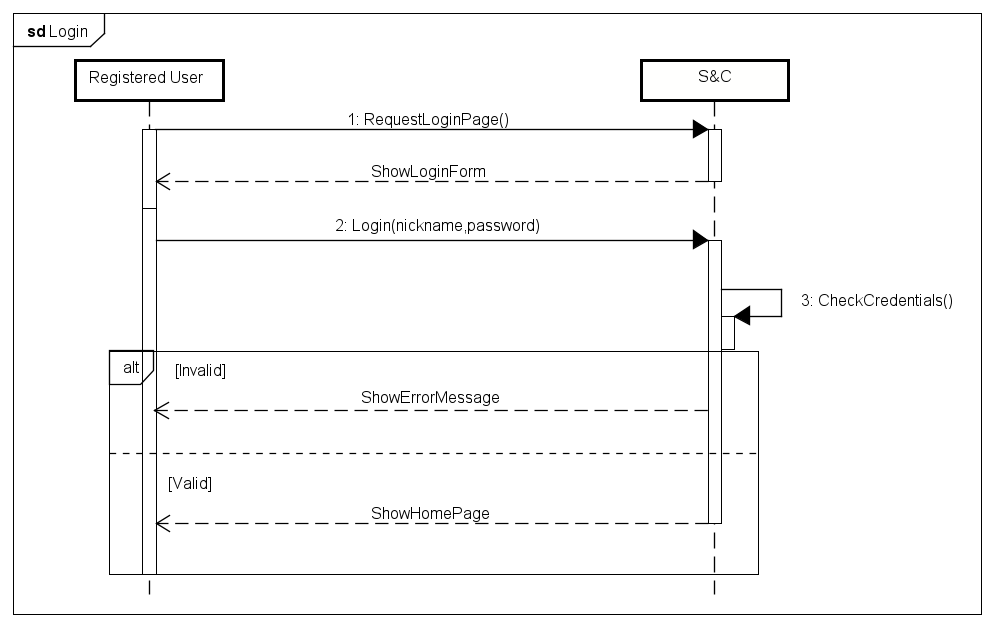
\includegraphics[width=1\linewidth]{Images/Sequence diagrams/Login.png}
    \caption{Login sequence diagram}
    \label{fig:enter-label}
\end{figure}

\textbf{UC\cuc\  - Student's account activation}

\begin{center} 
    \renewcommand{\arraystretch}{1.2} 
    \begin{longtable}{ l p{0.8\linewidth} } 
        \hline 
        Actor & Registered User \\ \hline 
        Entry Condition & The user wants to upgrade their account to a student account to unlock full access to the platform's features. \\ \hline 
        Event Flow & 1.\ The user presses the "Unlock full experience" button on the homepage. \\ 
        & 2.\ The user selects the "Student Account" option. \\  
        & 3.\ The user fills out all mandatory fields (name, surname, academic email, phone number, postal code). \\ 
        & 4.\ The user uploads their CV in PDF format. \\ 
        & 5.\ The user selects their internship goals from a provided checklist. \\ 
        & 6.\ The user presses the "Upgrade Account" button. \\ 
        & 7.\ The system validates the entered information and uploaded CV. \\ 
        & 8.\ If the information is valid, the system sends a confirmation email to verify the academic email's validity. \\ 
        & 9.\ The user clicks on the confirmation link in the email to complete the activation process. \\ \hline 
        Exit Condition & The user's account is successfully upgraded to a student account, granting access to additional features. \\ \hline 
        Exceptions & 1.\ One or more mandatory fields are left empty. \\ 
        & 2.\ The uploaded CV is not in the correct PDF format. \\ 
        & 3.\ The CV file is missing during the upload process. \\ 
        & 4.\ The entered information fails validation checks. \\
        & 5.\ An account with the provided academic email already exists. \\ \hline 
        \caption{User upgrades their account to a Student Account} 
        \label{tab:student_activation_uc} 
    \end{longtable} 
\end{center}

\begin{figure}[H]
    \centering
    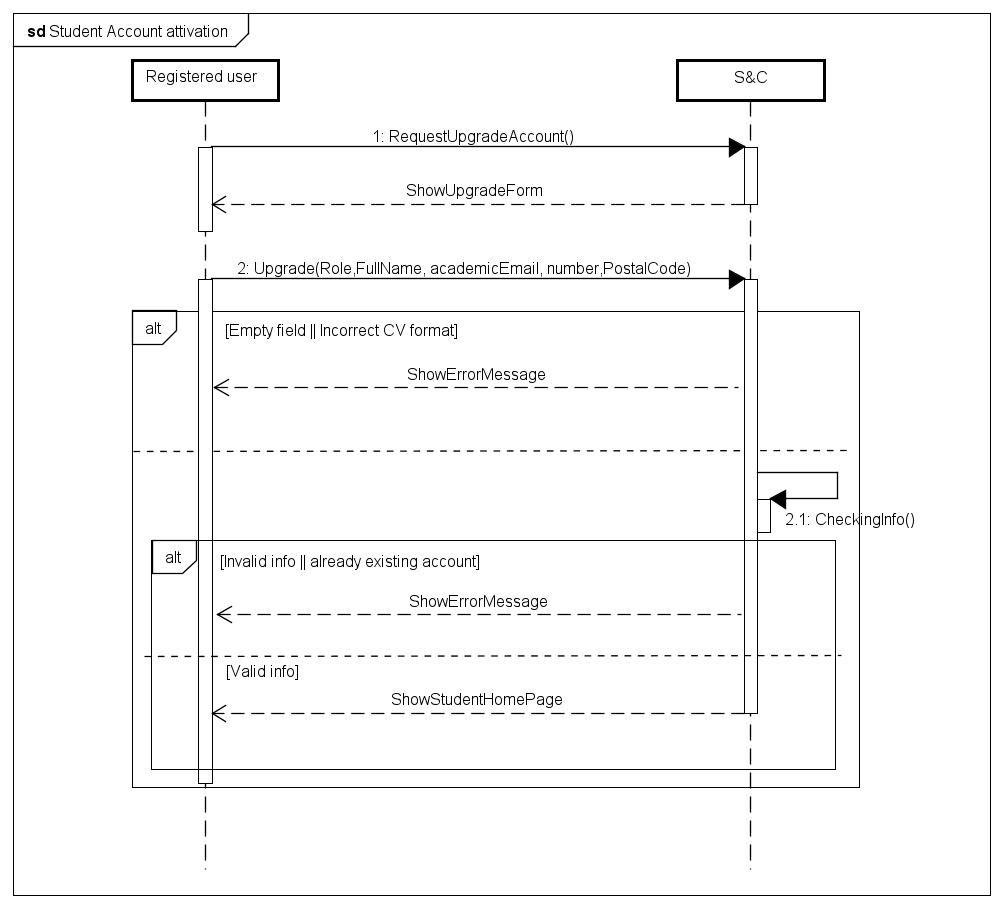
\includegraphics[width=1\linewidth]{Images/Sequence diagrams/Student account attivation.png}
    \caption{Student account activation sequence diagram}
    \label{fig:enter-label}
\end{figure}

\textbf{UC\cuc\  - Student modifies their profile or updates CV.}

\begin{center}
    \renewcommand{\arraystretch}{1.2}
    \begin{longtable}{ l p{0.8\linewidth} } 
        \hline
        Actor & Student \\ \hline
        Entry Condition & The student needs to modify their profile or wants to update their CV. \\ \hline
        Event Flow & 1.\ The student clicks on the "Profile" button. \\
        & 2.\ The student modifies the form with the correct data. \\
        & 2b.\ The student updates their CV with the suggestions offered by the S\&C system to ensure that the system can interpret the included data correctly. \\ 
        & 3.\ The student clicks on the "Update Profile" button. \\ \hline
        Exit Condition & The S\&C system registers the updated data and displays a success message. \\ \hline
        Exceptions & 1.\ One or more mandatory fields are left empty. \\ 
        & 2.\ The uploaded or updated CV is not in the correct PDF format. \\ 
        & 3.\ The entered information fails validation checks. \\ \hline
        \caption{Student updates their profile or CV.}
        \label{tab:student_profile_update_uc}%
    \end{longtable}
\end{center}

\begin{figure}[H]
    \centering
    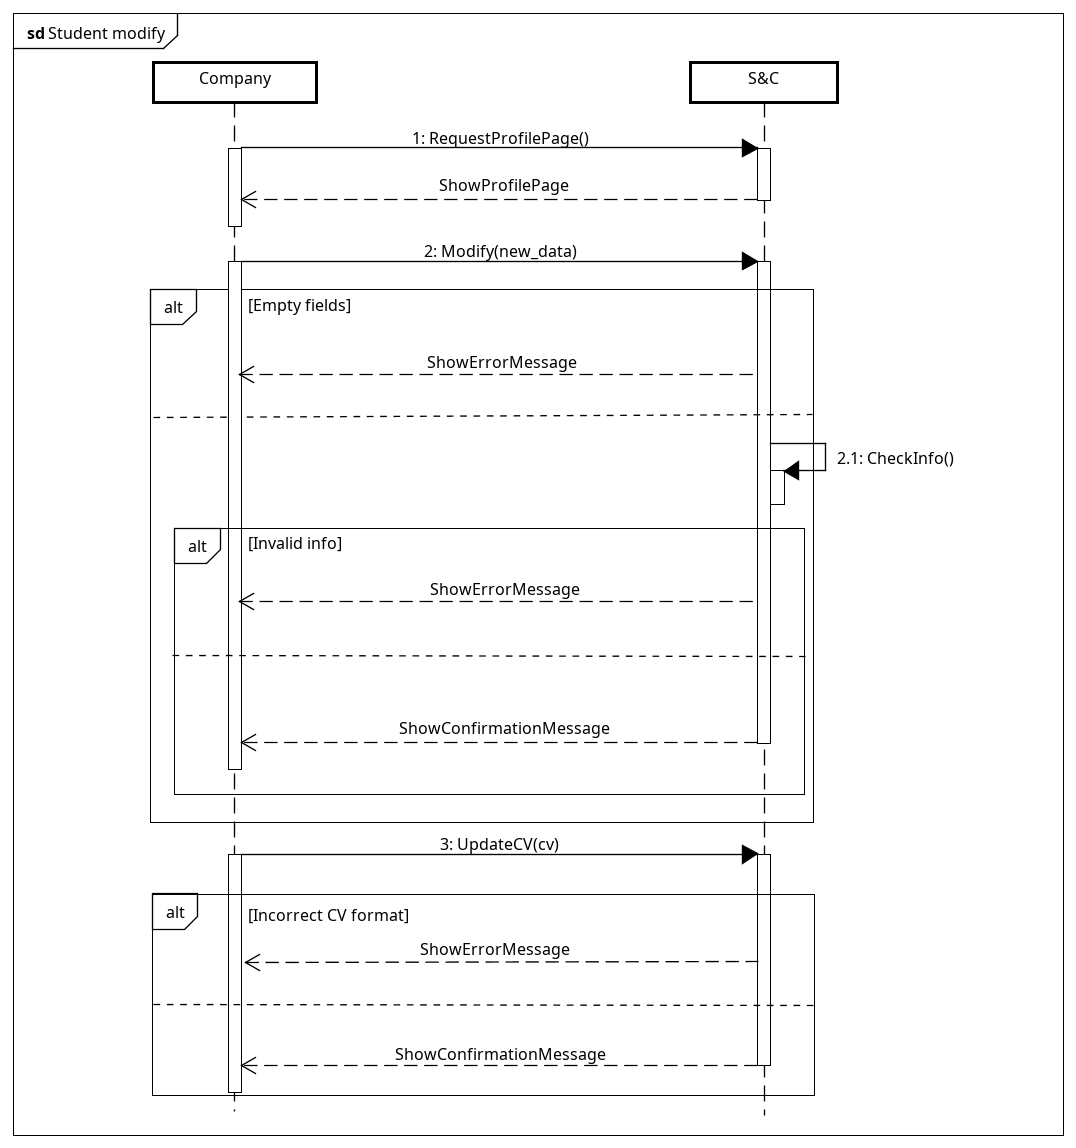
\includegraphics[width=1\linewidth]{Images/Sequence diagrams/Student modify.png}
    \caption{Student's profile update sequence diagram.}
    \label{fig:enter-label}
\end{figure}

\textbf{UC\cuc\  - Student checks available offers.}

\begin{center}
    \renewcommand{\arraystretch}{1.2}
    \begin{longtable}{ l p{0.8\linewidth} } 
        \hline
        Actor & Student \\ \hline
        Entry Condition & 1.\ The student logs in or he student clicks the "Home Page" button. \\ \hline
        Event Flow & 1.\ The student enters the S\&C system by logging in. \\
        & 2.\ If the student is on a different page, they click the "Home Page" button. \\ \hline
        Exit Condition & The S\&C system displays the student's personalized recommended internships. \\ \hline
        Exceptions & System error during page loading or redirection. \\ \hline
        \caption{Student checks available offers.}
        \label{tab:goals_tab}%
    \end{longtable}
\end{center}

\textbf{UC\cuc\  - Student opens details page of an internship post.}

\begin{center}
    \renewcommand{\arraystretch}{1.2}
    \begin{longtable}{ l p{0.8\linewidth} } 
        \hline
        Actor & Student \\ \hline
        Entry condition & Student clicks on the internship post.\\ \hline
        Event Flow       & 1.\ Student enters S\&C system logging in.\\ \hline
        Exit condition & S\&C system redirects shows student their personal recommended internships. \\ \hline
        Exceptions  & System cannot elaborate available internships.
        \\ \hline
        \caption{Student views offers.}
        \label{tab:goals_tab}%
    \end{longtable}
\end{center}

\textbf{UC\cuc\  - Student sends an application for an internship.}

\begin{center} 
    \renewcommand{\arraystretch}{1.2} 
    \begin{longtable}{ l p{0.8\linewidth} } 
        \hline 
        Actor & Student \\ \hline 
        Entry Condition & The student wants to apply for a specific internship offer. \\ \hline 
        Event Flow & 1.\ The student navigates to the internship offer by clicking on its box. \\ 
        & 2.\ The student clicks the "Apply to this internship" button. \\ 
        & 3.\ The system prompts for confirmation, and the student clicks the "Confirm" button to submit the application. \\ \hline 
        Exit Condition & The system displays a success message confirming that the application was submitted. \\ \hline 
        Exceptions & 1.\ The system is unable to process the application due to a technical issue. \\ 
        & 2.\ The internship offer is no longer available. \\ \hline 
        \caption{Student sends an application for an internship} 
        \label{tab:student_application_uc} 
    \end{longtable} 
\end{center}

\begin{figure}[H]
    \centering
    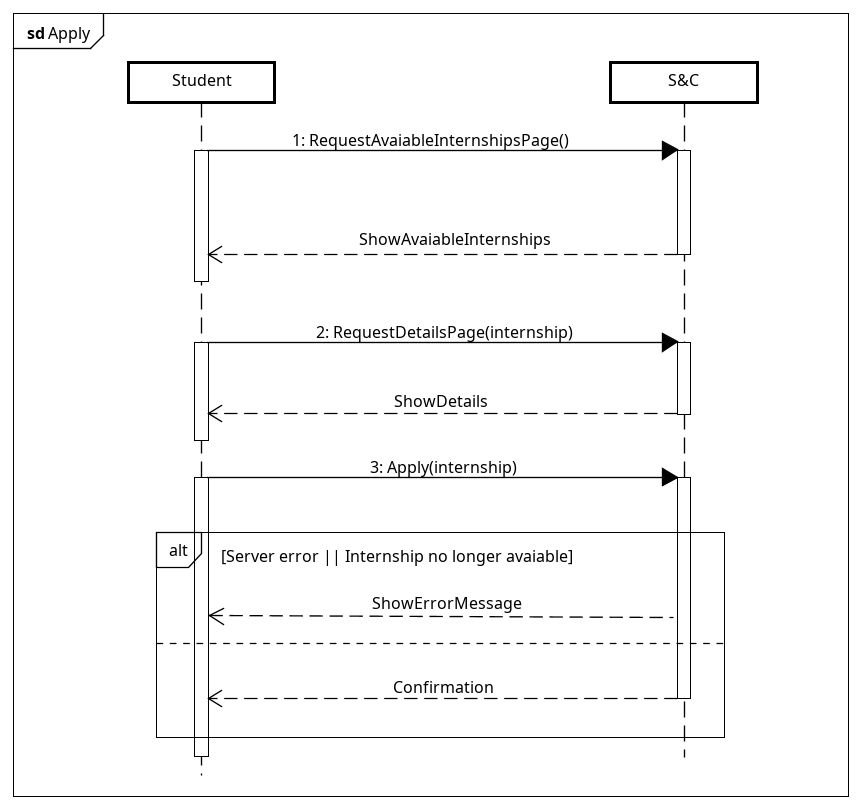
\includegraphics[width=1\linewidth]{Images/Sequence diagrams/Application.png}
    \caption{[UC 5-6-7] Student application sending path sequence diagram}
    \label{fig:enter-label}
\end{figure}

\textbf{UC\cuc\  - Student accepts or denies an interview schedule proposal from the company.}

\begin{center} 
    \renewcommand{\arraystretch}{1.2} 
    \begin{longtable}{ l p{0.8\linewidth} } 
        \hline
        Actor & Student \\ \hline
        Entry Condition & The student receives a notification about an interview schedule proposed by the company. \\ \hline 
        Event Flow & 1.\ The system sends a notification to the student about the interview schedule. \\ 
        & 2.\ The student clicks on the notification, opening a pop-up page displaying the schedule details. \\
        & 3.\ If the student agrees with the schedule, they click the "Accept" button. \\ 
        & 4.\ If the student disagrees, they provide a reason in the designated text field and click the "Deny" button. \\ \hline 
        Exit Condition & The system displays a confirmation message indicating that the student's decision (acceptance or denial) has been successfully registered. \\ \hline 
        Exceptions & 1.\ Schedule Not Available: The company cancels or updates the proposed schedule before the student views it. \\ \hline 
        \caption{Student accepts or denies an interview schedule proposal} 
        \label{tab:student_schedule_uc} 
    \end{longtable} 
\end{center}

\textbf{UC\cuc\  - Student accepts or denies the start of the internship.}

\begin{center} 
    \renewcommand{\arraystretch}{1.2} 
    \begin{longtable}{ l p{0.8\linewidth} } 
        \hline 
        Actor & Student \\ \hline 
        Entry Condition & The student receives a notification about the company's positive decision after the interview process. \\ \hline 
        Event Flow & 1.\ The system notifies the student of the company's decision to offer them the internship. \\ 
        & 2.\ The student clicks on the notification, opening a pop-up page with options to proceed. \\ 
        & 3.\ If the student agrees to start the internship, they click the "Confirm" button. \\ 
        & 4.\ If the student declines the offer, they provide a reason in the designated text field and click the "Deny" button. \\ \hline 
        Exit Condition & The system registers the student's decision (acceptance or denial) and displays a success message confirming the action. \\ \hline 
        \caption{Student Accepts or Denies the Start of an Internship} 
        \label{tab:student_internship_uc} 
    \end{longtable} 
\end{center}

\begin{figure}[H]
    \centering
    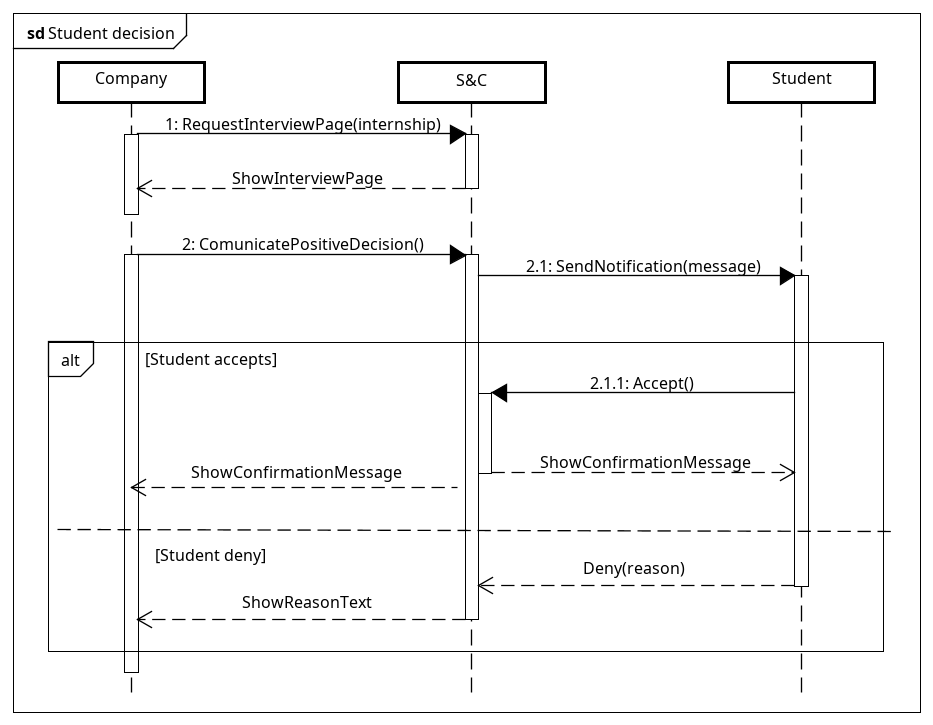
\includegraphics[width=1\linewidth]{Images/Sequence diagrams/Student decision.png}
    \caption{Student's response to internship proposal sequence diagram}
    \label{fig:enter-label}
\end{figure}

\textbf{UC\cuc\  - Company's account activation}

\begin{center} 
    \renewcommand{\arraystretch}{1.2} 
    \begin{longtable}{ l p{0.8\linewidth} } 
        \hline 
        Actor & Registered User \\ \hline 
        Entry Condition & The user wants to upgrade their account to a company account to unlock full access to the platform's features. \\ \hline 
        Event Flow & 1.\ The user presses the "Unlock full experience" button on the homepage. \\ 
        & 2.\ The user selects the "Company Account" option. \\ 
        & 3.\ The user fills in all mandatory fields (full name, phone number, office address). \\ 
        & 4.\ The user presses the "Upgrade Account" button. \\ 
        & 5.\ The system validates the entered information. \\ \hline 
        Exit Condition & The user's account is successfully upgraded to a company account, granting access to additional features. \\ \hline 
        Exceptions & 1.\ One or more mandatory fields are left empty. \\ 
        & 2.\ The entered information fails validation checks. \\ \hline 
        \caption{User upgrades their account to a Company Account} 
        \label{tab:company_activation_uc} 
    \end{longtable} 
\end{center}

\begin{figure}[H]
    \centering
    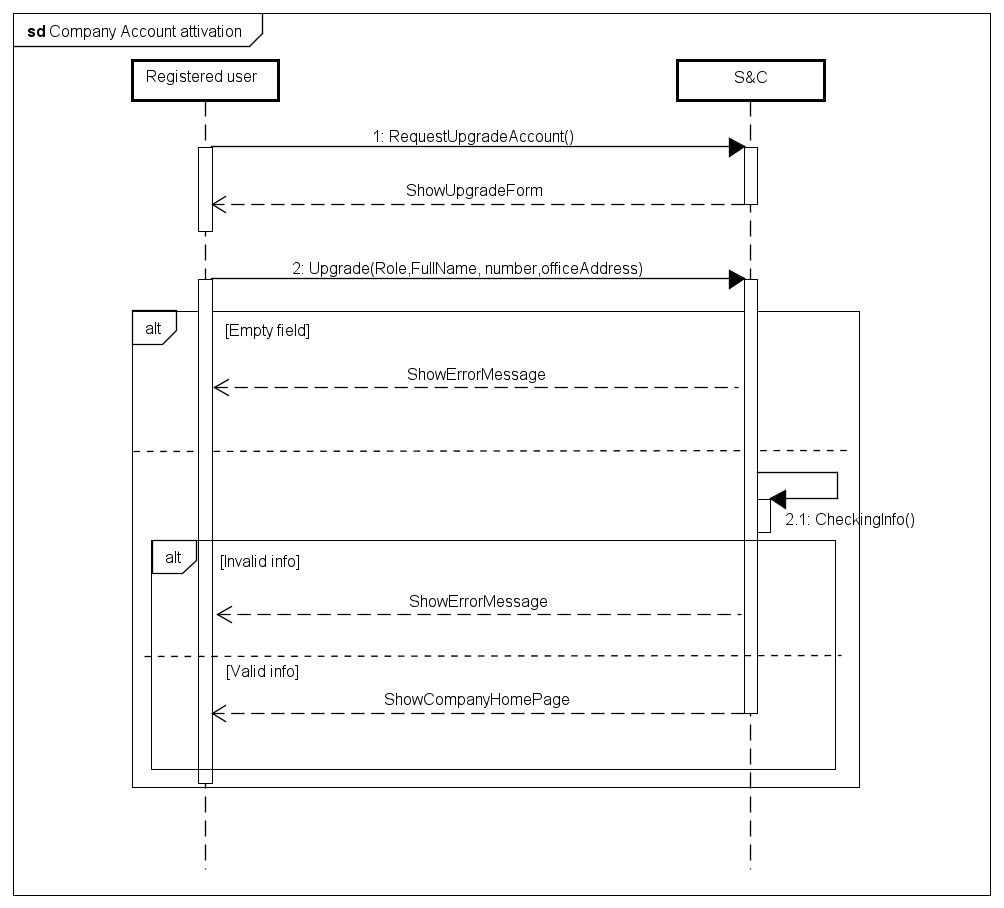
\includegraphics[width=1\linewidth]{Images/Sequence diagrams/Company Account attivation.png}
    \caption{Student account activation sequence diagram}
    \label{fig:enter-label}
\end{figure}

\textbf{UC\cuc\  - Company modifies their profile.}

\begin{center}
    \renewcommand{\arraystretch}{1.2}
    \begin{longtable}{ l p{0.8\linewidth} } 
        \hline
        Actor & Company \\ \hline
        Entry Condition & The company needs to update their profile because some information is incorrect or out of date. \\ \hline
        Event Flow & 1.\ The company clicks on the "Profile" button. \\
        & 2.\ The company modifies the form with the correct data. \\
        & 3.\ The company clicks on the "Update Profile" button. \\ \hline
        Exit Condition & The S\&C system registers the updated data and displays a success message. \\ \hline
        Exceptions & 1.\ One or more mandatory fields are left empty. \\
        & 2.\ The entered information fails validation checks. \\ \hline
        \caption{Company updates their profile.}
        \label{tab:company_profile_update_uc}%
    \end{longtable}
\end{center}

\begin{figure}[H]
    \centering
    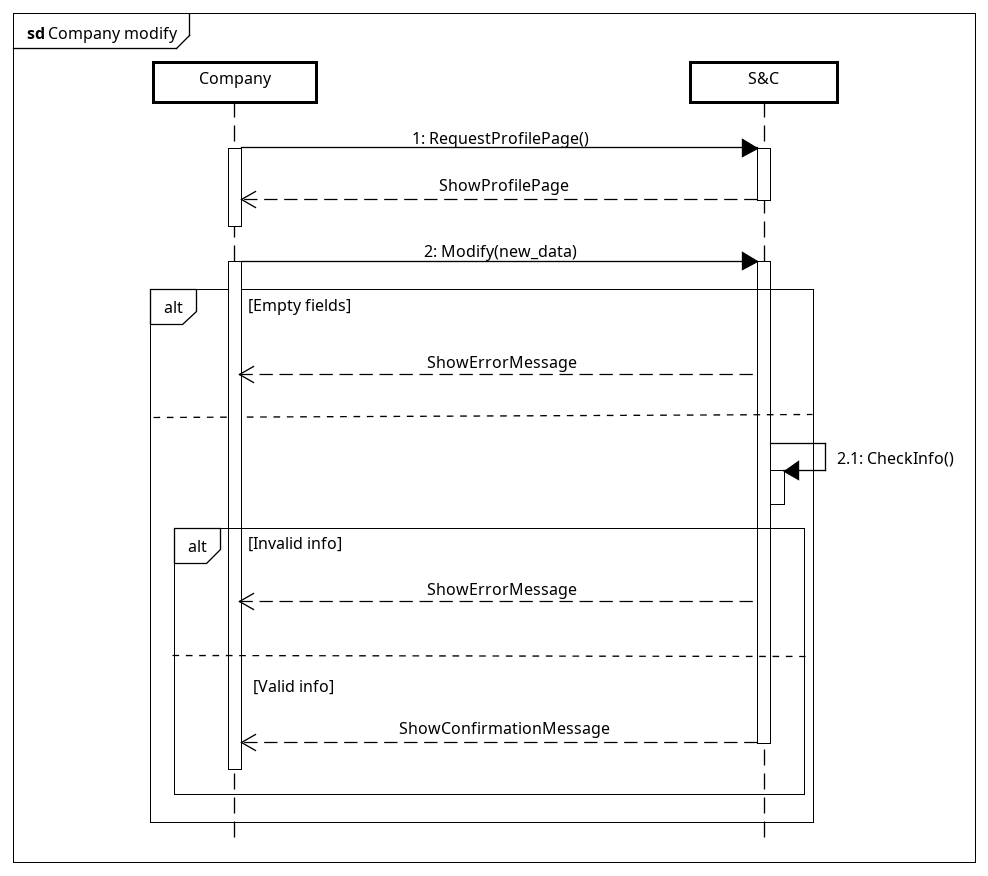
\includegraphics[width=1\linewidth]{Images/Sequence diagrams/Company modify.png}
    \caption{Company's profile update sequence diagram}
    \label{fig:enter-label}
\end{figure}

\textbf{UC\cuc\  - Company posts a new internship offer}

\begin{center} 
    \renewcommand{\arraystretch}{1.2} 
    \begin{longtable}{ l p{0.8\linewidth} } 
        \hline 
        Actor & Company \\ \hline 
        Entry Condition & The company decides to create and publish a new internship offer to attract suitable candidates. \\ \hline Event Flow & 1.\ The company presses the "+" button on the homepage. \\ 
        & 2.\ The company fills out the internship offer form, inserting project description, requested role, location address (if different from the default office address), salary (if applicable), number of students (if more than one is required), skills the student will gain, weekly schedule, benefits offered as mentorship, training opportunities, etc. This process is assisted by system-generated suggestions designed to make the post more appealing and engaging for students \\ 
        & 3.\ The company reviews the information and clicks the "Post offer" button. \\ \hline 
        Exit Condition & The system successfully registers the new internship offer and displays a confirmation message. The offer becomes visible to students. \\ \hline 
        Exceptions & 1.\ One or more mandatory fields in the form are left empty.\\ \hline 
        \caption{Company posts a new internship offer} 
        \label{tab:company_post_offer_uc} 
    \end{longtable} 
\end{center}

\begin{figure}[H]
    \centering
    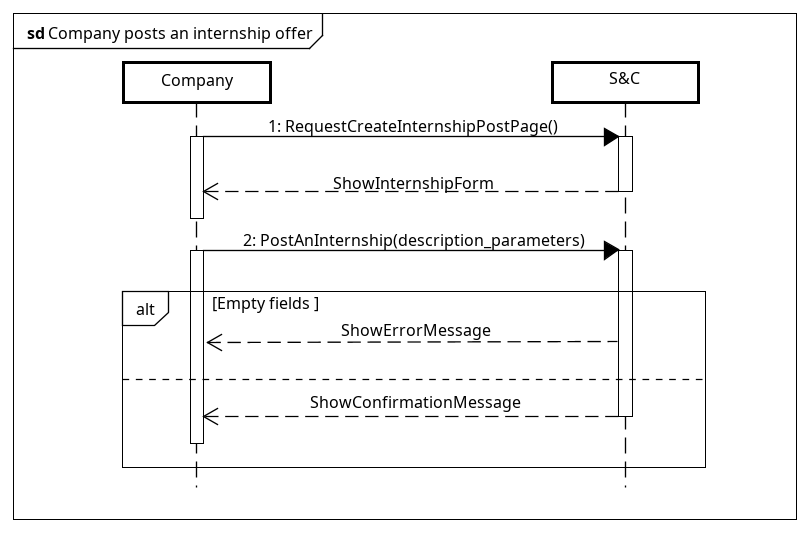
\includegraphics[width=1\linewidth]{Images/Sequence diagrams/Company posts an internship offer.png}
    \caption{Company internship post creation sequence diagram}
    \label{fig:enter-label}
\end{figure}

\textbf{UC\cuc\  - The company accepts an application or identifies a promising student and proposes a schedule for the interview}

\begin{center} 
    \renewcommand{\arraystretch}{1.2} 
    \begin{longtable}{ l p{0.8\linewidth} } 
        \hline 
        Actor & Company \\ \hline 
        Entry Condition & 1.\ The company is notified about a new application from a suitable student. \\ 
        & 2.\ The company decides to accept an application from a student. \\ 
        & 3.\ The company identifies a promising student directly from the system, even if the student has not sent an application. \\ \hline 
        Event Flow &  1.\ The company clicks on the notification received about a matching student's application. \\
        & 1b.\ Alternatively, the company navigates to the internship offer, clicks on the its box and selects the student's profile. \\ 
        & 1c.\ As another option, the company searches for the student’s profile from the internship offer and selects it. \\ 
        & 2.\ The system displays the student’s detailed profile page. \\ 
        & 3.\ The company clicks the "Propose interview" or "Contact student" button. \\ 
        & 4.\ A pop-up form appears, allowing the company to schedule an interview. \\ 
        & 5.\ The company completes the form with details such as date and time of the interview, format (in-person, video call), additional comments or instructions (if any). \\ 
        & 6.\ The company clicks the "Send proposal" button. \\ \hline 
        Exit Condition & The system successfully registers the interview proposal and notifies the student. A confirmation message is displayed to the company. \\ \hline 
        Exceptions & 1.\ One or more mandatory fields in the interview scheduling form are left empty. \\ 
        & 2.\ The student is already engaged in another internship or is unavailable. \\ \hline
        \caption{The company accepts an application or identifies a promising student and proposes a schedule for the interview} 
        \label{tab:company_post_offer_uc} 
    \end{longtable} 
\end{center}

\begin{figure}[H]
    \centering
    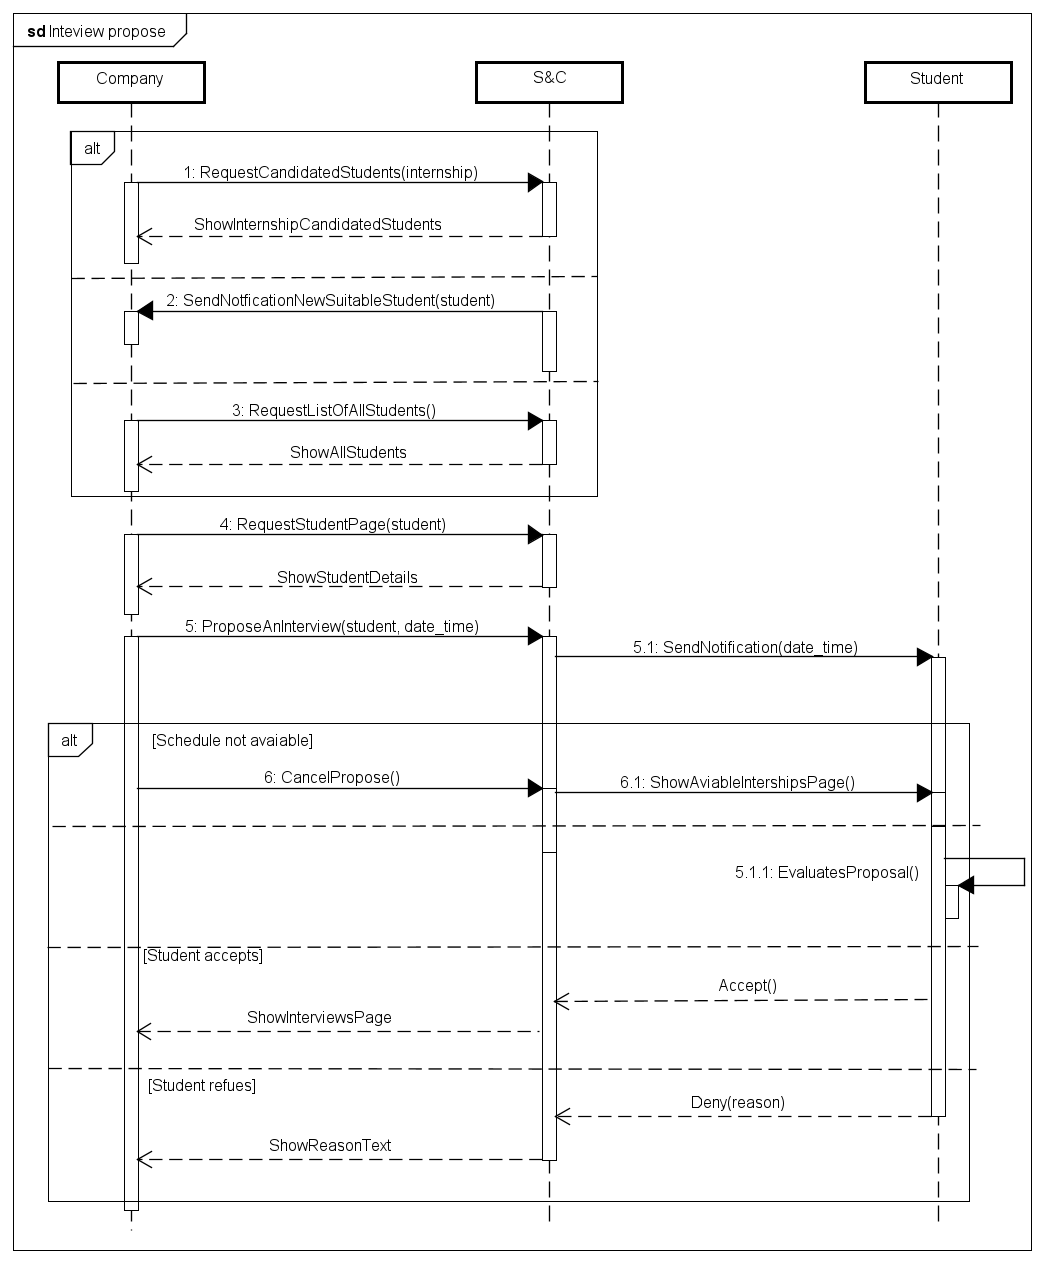
\includegraphics[width=1\linewidth]{Images/Sequence diagrams/Inteview propose.png}
    \caption{[UC 8-13] Interview propose path sequence diagram}
    \label{fig:enter-label}
\end{figure}

\textbf{UC\cuc\  - Student or Company submits a complaint about an ongoing internship.}

\begin{center} 
    \renewcommand{\arraystretch}{1.2} 
    \begin{longtable}{ l p{0.8\linewidth} } 
        \hline Actor & Student or Company \\ \hline 
        Entry Condition & The actor identifies a problem or negative aspect of their ongoing internship and wants to notify the university. \\ \hline 
        Event Flow & 1.\ The actor navigates to the "ongoing internship" tab. \\  
        & 2.\ The actor fills out the complaint form, providing details about the issue. \\ 
        & 3.\ The actor clicks the "Submit" button to send the complaint. \\ \hline 
        Exit Condition & The system successfully registers the complaint and confirms its submission to the university. \\ \hline
        \caption{Student or Company submits a complaint about an ongoing internship} 
        \label{tab:student_complaint_uc} 
    \end{longtable} 
\end{center}

\begin{figure}[H]
    \centering
    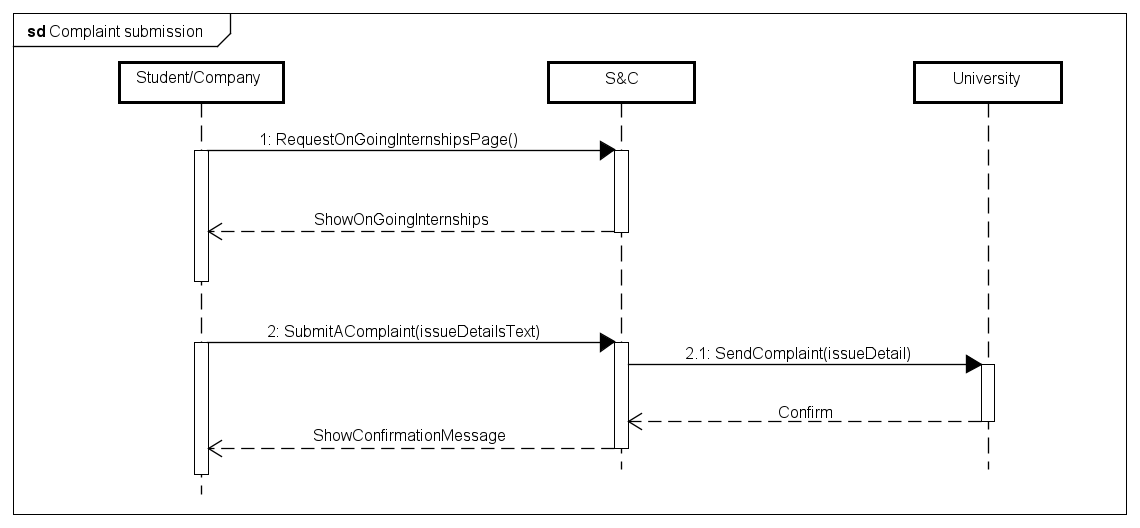
\includegraphics[width=1\linewidth]{Images/Sequence diagrams/Complaint submission.png}
    \caption{Student/Company complaint submission sequence diagram}
    \label{fig:enter-label}
\end{figure}

\textbf{UC\cuc\  - Student or Company submits a feedback about a terminated internship.}

\begin{center} 
    \renewcommand{\arraystretch}{1.2} 
    \begin{longtable}{ l p{0.8\linewidth} } 
        \hline 
        Actor & Student or Company \\ \hline 
        Entry Condition & The internship has been terminated and an actor wants to provide feedback to help improve the system's recommendations. \\ \hline 
        Event Flow & 1.\ The actor navigates to the "terminated internships" section. \\
        & 2.\ The actor selects the relevant internship from the list. \\
        & 3.\ The actor fills out the feedback form, providing details about their experience, including pros, cons, and suggestions. \\
        & 4.\ The actor clicks the "Submit feedback" button to send it. \\ \hline 
        Exit Condition & The system successfully registers the actor's feedback, which is used to refine the recommendation algorithm and enhance future matches. \\ \hline  
        \caption{Student or Company submits feedback about a terminated internship} 
        \label{tab:student_feedback_uc} 
    \end{longtable} 
\end{center}

\begin{figure}[H]
    \centering
    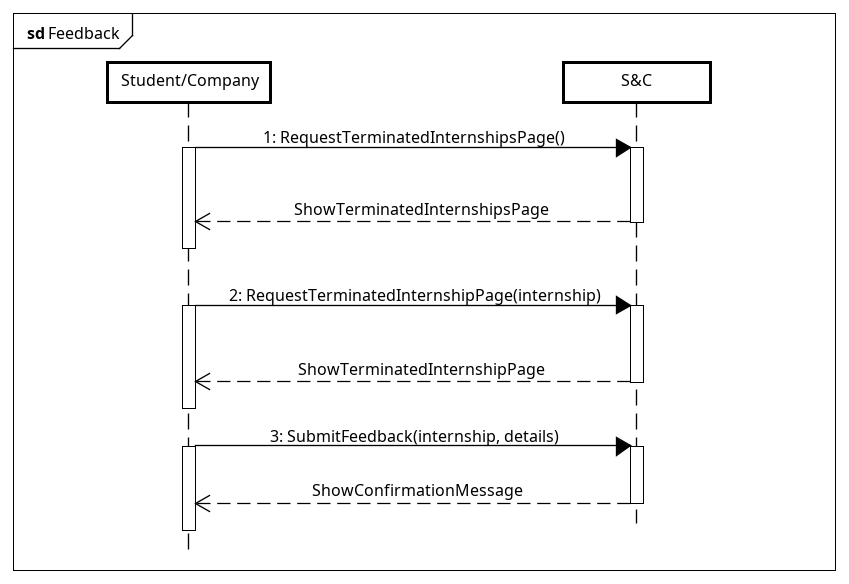
\includegraphics[width=1\linewidth]{Images/Sequence diagrams/Feedback.png}
    \caption{Student/Company feedback submission sequence diagram}
    \label{fig:enter-label}
\end{figure}

\textbf{UC\cuc\  - University decides to interrupt an internship due to relevant complaints.}

\begin{center} 
    \renewcommand{\arraystretch}{1.2} 
    \begin{longtable}{ l p{0.8\linewidth} } 
        \hline 
        Actor & University \\ \hline 
        Entry Condition & 1.\ The university is notified about a complaint concerning an ongoing internship. \\ 
        & 2.\ The university determines that the issue reported is significant enough to warrant the termination of the internship. \\ \hline
        Event Flow &  1.\ The university clicks on the notification related to the complaint. \\ 
        & 1b.\ Alternatively, the university navigates to the "Current internships" list and selects the internship. \\ 
        & 2.\ The system displays the details of the internship and the associated complaint(s). \\ 
        & 3.\ The university clicks the "Interrupt internship" button. \\ 
        & 4.\ A confirmation pop-up appears, and the university provides a reason for the interruption in a text field. \\ 
        & 5.\ The university clicks "Confirm" to finalize the decision. \\ \hline 
        Exit Condition & The system successfully registers the decision and sends notifications to both the company and the student, detailing the reason for the termination. \\ \hline
        \caption{University Decides to Interrupt an Internship Due to Relevant Complaints} 
        \label{tab:university_interrupt_uc} 
    \end{longtable} 
\end{center}

\begin{figure}[H]
    \centering
    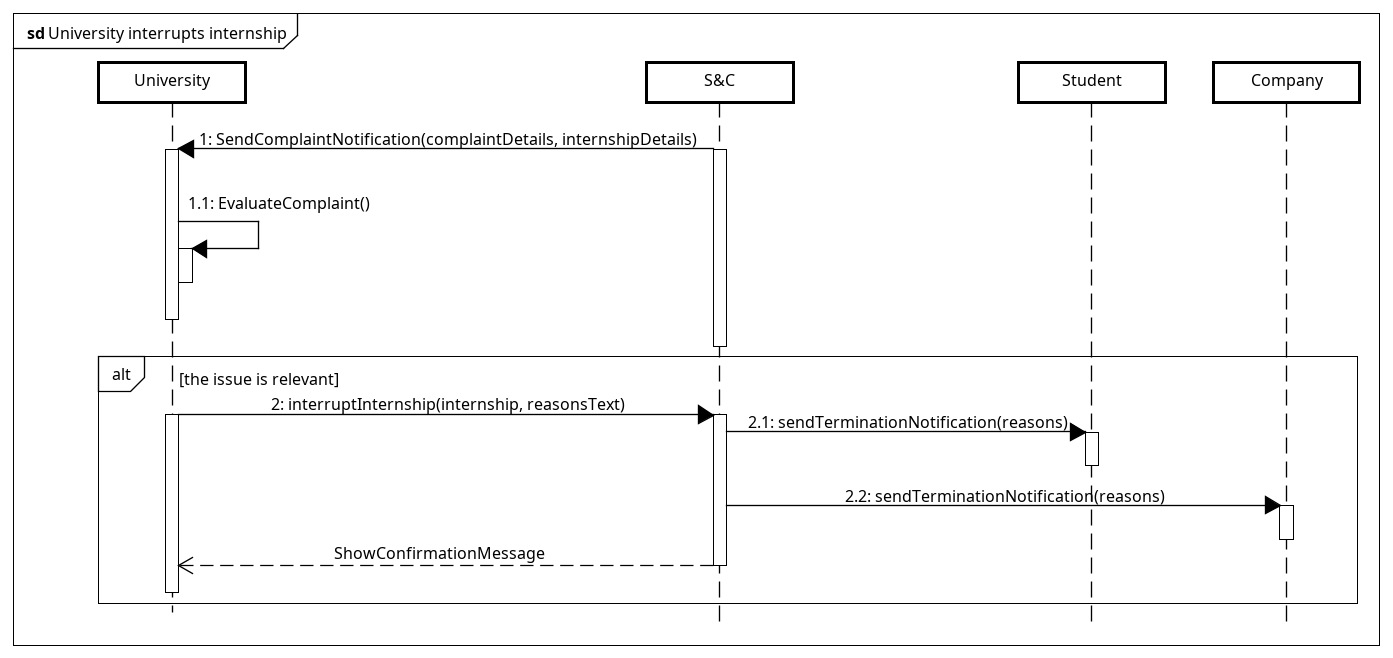
\includegraphics[width=1\linewidth]{Images/Sequence diagrams/University interrupts internship.png}
    \caption{University internship interrupt sequence diagram}
    \label{fig:enter-label}
\end{figure}


\clearpage

\subsection{Mapping on goals}
\label{subsec: map_on_g}%

\begin{itemize}
    \item \textbf{G1 - Allows Companies to advertise their internship offers to find the most suitable students, with the help of recommendation.}
    \begin{itemize}
        \item R1: S\&C system allows unregistered users to sign-up.
        \item R2: S\&C system allows registered users to verify their email address.
        \item R6: S\&C system allows registered users to view posted internships on the platform.
        \item R27: S\&C system allows Companies to post internship offers by providing detailed information.
        \item R28: S\&C system allows Companies to edit an internship's post.
        \item R29: S\&C system allows Companies to delete an internship's post.
        \item R30: S\&C system allows Companies to identify the most suitable students on the platform for their internship posts, even if the students have not applied.
        \item R47: S\&C system periodically updates internship recommendations based on new data from Students and Companies.
    \end{itemize}
    \item \textbf{G2 - Allows Students to look for internships based on their needs and find the most suitable for them, with the help of recommendation.}
    \begin{itemize}
        \item R4: S\&C system allows registered users to edit their account details.
        \item R7: S\&C system allows registered users to upgrade to a Student account or a Company account.
        \item R9: S\&C system allows registered users to update their notifications preferences.
        \item R10: S\&C system allows Students to view a personalized dashboard in their homepage.
        \item R11: S\&C system allows Students to explore available internships.
        \item R12: S\&C system allows Students to view available internships ordered by the best matching, based on a matching score system.
        \item R13: S\&C system allows Students to change the default order.
        \item R14: S\&C system allows Students to apply filters on the view of the available internships.
        \item R15: S\&C system allows Students to receive notification when a new internship matching their profile is posted.
        \item R16: S\&C system allows Students to view the details of a specific internship page.
        \item R33: S\&C system allows Companies to receive notification when a new student with a high matching score has applied.
        \item R46: S\&C system improves recommendation accuracy by considering user feedback on previous internships.
        \item R47: S\&C system periodically updates internship recommendations based on new data from Students and Companies.
    \end{itemize}
    \item \textbf{G3 - Supports selection process by helping manage interviews and also finalize the selections.}
    \begin{itemize}
        \item R17: S\&C system allows Students to apply for an internship.
        \item R18: S\&C system allows Students to view sent applications.
        \item R19: S\&C system allows Students to monitor the status of an application.
        \item R20: S\&C system allows Students to withdraw a sent application.
        \item R21: S\&C system allows Students to confirm their participation of a scheduled interview via a notification interface.
        \item R22: S\&C system allows Students to decline an interview offer via a notification interface.
        \item R31: S\&C system allows Companies to review the applications for an internship.
        \item R32: S\&C system allows Companies to view internship's applications ordered by the best match.
        \item R34: S\&C system allows Companies to propose a date to a student to schedule an interview.
        \item R35: S\&C system allows Companies to prepare a standardized set of questions to be proposed to all candidates for a specific internship.
        \item R36: S\&C system allows Companies to compare the answers from all candidates to facilitate the selection process.
        \item R37: S\&C system allows Companies to reject a student after the interview.
    \end{itemize}
    \item \textbf{G4 - Provides suggestions to companies regarding how to make their offers more appealing for students.}
    \begin{itemize}
        \item R27: S\&C system allows Companies to post internship offers by providing detailed information.
        \item R46: S\&C system improves recommendation accuracy by considering user feedback on previous internships.
    \end{itemize}
    \item \textbf{G5 - Provides suggestions to students how to make their CVs more appealing for companies.}
    \begin{itemize}
        \item R8: S\&C system allows registered users to verify their current academic status by validating their institutional email address.
        \item R24: S\&C system allows Students to review the agreements of an internship before accepting.
    \end{itemize}
    \item \textbf{G6 - Allows stakeholders to monitor the progress of internships, report issues, and track outcomes.}
    \begin{itemize}
        \item R5: S\&C system allows registered users to delete their account.
        \item R23: S\&C system sends automated reminders to Students for upcoming interview deadlines.
        \item R26: S\&C system allows Students to submit feedback after completing an internship.
        \item R38: S\&C system allows Companies to start an internship.
        \item R39: S\&C system allows Companies to view active internships.
        \item R40: S\&C system allows Companies to file a complaint.
        \item R41: S\&C system allows Companies to submit feedback after completing an internship.
        \item R43: S\&C system allows universities to collect complaints raised by Students.
        \item R44: S\&C system allows universities to collect complaints raised by Companies.
    \end{itemize}

    
    \item \textbf{G7 - Allows Universities to monitor the situation of ongoing internships and interrupt them when necessary.}
    \begin{itemize}
        \item R3: S\&C system allows registered users to login.
        \item R25: S\&C system allows Students to file a complaint.
        \item R42: S\&C system allows universities to login to the system providing credentials.
        \item R45: S\&C system allows universities to mediate between Student and Company after a complaint.
    \end{itemize}
\end{itemize}

\clearpage

\renewcommand{\arraystretch}{1.5}
    \begin{longtable}{|l|c|c|c|c|c|c|c|}
        \hline
        \textbf{Requirement} & \textbf{G1} & \textbf{G2} & \textbf{G3} & \textbf{G4} & \textbf{G5} & \textbf{G6} & \textbf{G7} \\
        \hline
            R1  & \checkmark &   &   &   &   &   &   \\ \hline
            R2  & \checkmark &   &   &   &   &   &   \\ \hline
            R3  &   &   &   &   &   &   & \checkmark \\ \hline
            R4  &   & \checkmark &   &   &   &   &   \\ \hline
            R5  &   &   &   &   &   & \checkmark &   \\ \hline
            R6  & \checkmark &   &   &   &   &   &   \\ \hline
            R7  &   & \checkmark &   &   &   &   &   \\ \hline
            R8  &   &   &   &   & \checkmark &   &   \\ \hline
            R9  &   & \checkmark &   &   &   &   &   \\ \hline
            R10 &   & \checkmark &   &   &   &   &   \\ \hline
            R11 &   & \checkmark &   &   &   &   &   \\ \hline
            R12 &   & \checkmark &   &   &   &   &   \\ \hline
            R13 &   & \checkmark &   &   &   &   &   \\ \hline
            R14 &   & \checkmark &   &   &   &   &   \\ \hline
            R15 &   & \checkmark &   &   &   &   &   \\ \hline
            R16 &   & \checkmark &   &   &   &   &   \\ \hline
            R17 &   &   & \checkmark &   &   &   &   \\ \hline
            R18 &   &   & \checkmark &   &   &   &   \\ \hline
            R19 &   &   & \checkmark &   &   &   &   \\ \hline
            R20 &   &   & \checkmark &   &   &   &   \\ \hline
            R21 &   &   & \checkmark &   &   &   &   \\ \hline
            R22 &   &   & \checkmark &   &   &   &   \\ \hline
            R23 &   &   &   &   &   & \checkmark &   \\ \hline
            R24 &   &   &   &   & \checkmark &   &   \\ \hline
            R25 &   &   &   &   &   &   & \checkmark \\ \hline
            R26 &   &   &   &   &   & \checkmark &   \\ \hline
            R27 & \checkmark &   &   & \checkmark &   &   &   \\ \hline
            R28 & \checkmark &   &   &   &   &   &   \\ \hline
            R29 & \checkmark &   &   &   &   &   &   \\ \hline
            R30 & \checkmark &   &   &   &   &   &   \\ \hline
            R31 &   &   & \checkmark &   &   &   &   \\ \hline
            R32 &   &   & \checkmark &   &   &   &   \\ \hline
            R33 &   & \checkmark &   &   &   &   &   \\ \hline
            R34 &   &   & \checkmark &   &   &   &   \\ \hline
            R35 &   &   & \checkmark &   &   &   &   \\ \hline
            R36 &   &   & \checkmark &   &   &   &   \\ \hline
            R37 &   &   & \checkmark &   &   &   &   \\ \hline
            R38 &   &   &   &   &   & \checkmark &   \\ \hline
            R39 &   &   &   &   &   & \checkmark &   \\ \hline
            R40 &   &   &   &   &   & \checkmark &   \\ \hline
            R41 &   &   &   &   &   & \checkmark &   \\ \hline
            R42 &   &   &   &   &   &   & \checkmark \\ \hline
            R43 &   &   &   &   &   & \checkmark &   \\ \hline
            R44 &   &   &   &   &   & \checkmark &   \\ \hline
            R45 &   &   &   &   &   &   & \checkmark \\ \hline
            R46 &   & \checkmark &   & \checkmark &   &   &   \\ \hline
            R47 & \checkmark & \checkmark &   &   &   &   &   \\ \hline
        \caption{ Traceability Matrix for Goals and Requirements}
    \end{longtable}
\label{tab:mapping_requirements}



\section{Performance Requirements}
\label{sec:performance_requirements}%
The platform has to guarantee good performances in order to work efficiently and correctly for a great number of users (Universities, Students and Companies). In order to achieve this the response time must be lower than a second, this is due to the fact that the user's connection to the platform can be slow and the loading times can subsequently increase in an exponential way.

\section{Design Constraints}
\label{sec:performance_requirements}%

\subsection{Standard compliance}
\label{subsec: standard_compliance}%
The S\&C platform adheres to regulations and standards to ensure data privacy and usability. It complies with the General Data Protection Regulation (GDPR) for secure handling of personal data, including student CVs and company profiles. Additionally, all communications use HTTPS to guarantee secure data transmission, and the international format for date and time is adopted to ensure clarity and consistency across different regions. 
\subsection{Hardware limitations}
\label{subsec: hardware_limitations}%
Here we have a short list of the hardware features that a user should have to use the platform without encountering major problems:
\begin{itemize}
    \item The user must have a device with a good internet connection this means that the device in question should be compatible with at least one of the following standards : 3G, 4G, 5G, IEEE 802.11 or IEEE 802.3. Both wired and wireless connections must be guaranteed during the usage of the platform.
    \item The user must have a device with good hardware features such as a processor with high performance 
\end{itemize}
 
\subsection{Any Other Constraint}
\label{subsec: hardware_limitations}%
In a way, the system ought to give top priority to how user-friendly it is, providing interfaces that feel easy to learn for students, companies, and universities alike for things like uploading resumes, handling internships, and sorting out complaints. It must integrate efficiently with third-party tools (e.g., video conferencing softwares) and ensure compatibility with APIs that support future features (e.g. AI-based recommendations).  The architecture must be as scalable as the platform itself increases in the number of users. The platform should also be integrated with specific tools in order to make the feedback and complaint system robust.
\section{Software system attributes}
\label{sec:performance_requirements}%

\subsection{Reliability}
\label{subsec: reliability}%
The system has to be reliable since it will have to run without stopping for a long period of time. To ensure this feature the platform must have some sort of replication and consistency policy to avoid system crash. In addition to this it is a good practice to have offline backups of the system for recovering information in case of data loss. 
\subsection{Availability}
\label{subsec: availability}%
The system must guarantee an availability of 99\% to support its users effectively, especially during peak usage periods like internship deadlines or videoconferencing sessions. To achieve this, single points of failure must be avoided and load balancing techniques should be used. 
\subsection{Security}
\label{subsec: security }%
User data, including personal information and CVs, must be protected using encryption methods for stored data and secure transmission protocols. The platform must implement measures to prevent unauthorized access and ensure the integrity and confidentiality of user information. 
\subsection{Maintainability}
\label{subsec: maintainability}%
The system must be easily maintainable with well-documented code and routine testing procedures. At least 75\% of the code, excluding the UI, must have test coverage to facilitate debugging and future development and expansion of the platform. 
\subsection{Portability}
\label{subsec: portability}%
As a web-based application, the platform must work correctly on various devices and browsers, such as Chrome, Firefox, and Safari. Compatibility with both desktop and mobile devices ensures usability for a wide range of users. 


    \chapter{Formal Analysis Using Alloy}
    \label{ch:formal_analysis_using_alloy}%
    \section{Objectives of the analysis}
In this section, a presentation of the formal modeling activity has been created using the Alloy formal notation with the main goal of describing the domain and the properties of the system. 
The objective of this is to model and formally represent all the users (University, Student, Company, and regular User) and everything related to Internships and Internship Offers as well as the main constraints which regard all the entities mentioned.
\vspace{0.5cm}
\lstinputlisting[language=alloy]{Alloy/RASD_ALLOY.als}
\newpage
\section{Metamodels and Examples}
\subsection{General}
This model shows the entire system and all the complex relations among its parts. It can be quite useful to better understand how the single parts interact with each other.
\begin{figure}[H]
    \centering
    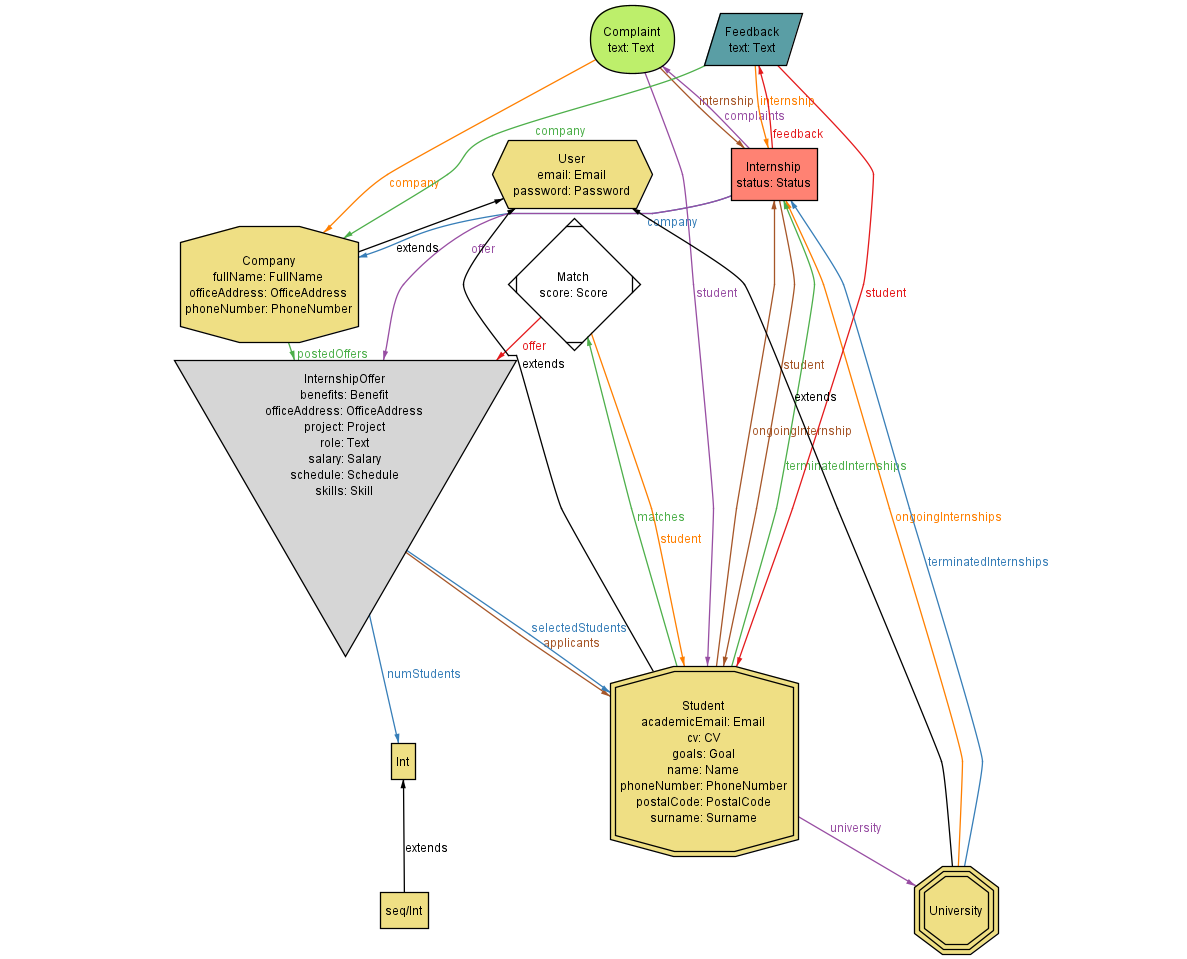
\includegraphics[width=0.75\linewidth]{Images/Alloy/metamodel.png}
    \caption{metamodel of the entire system }
    \label{fig:enter-label}
\end{figure}
\subsection{Users}
This model describes the basic properties of each user, independently from their type (University, Company, Student), without making any connection to other entities.
From this model the concept of the user who doesn't belong to one of the three groups that are able to interact with the platform is removed because it can not have relationships with any of the entities in the system.
\begin{figure}
    \centering
    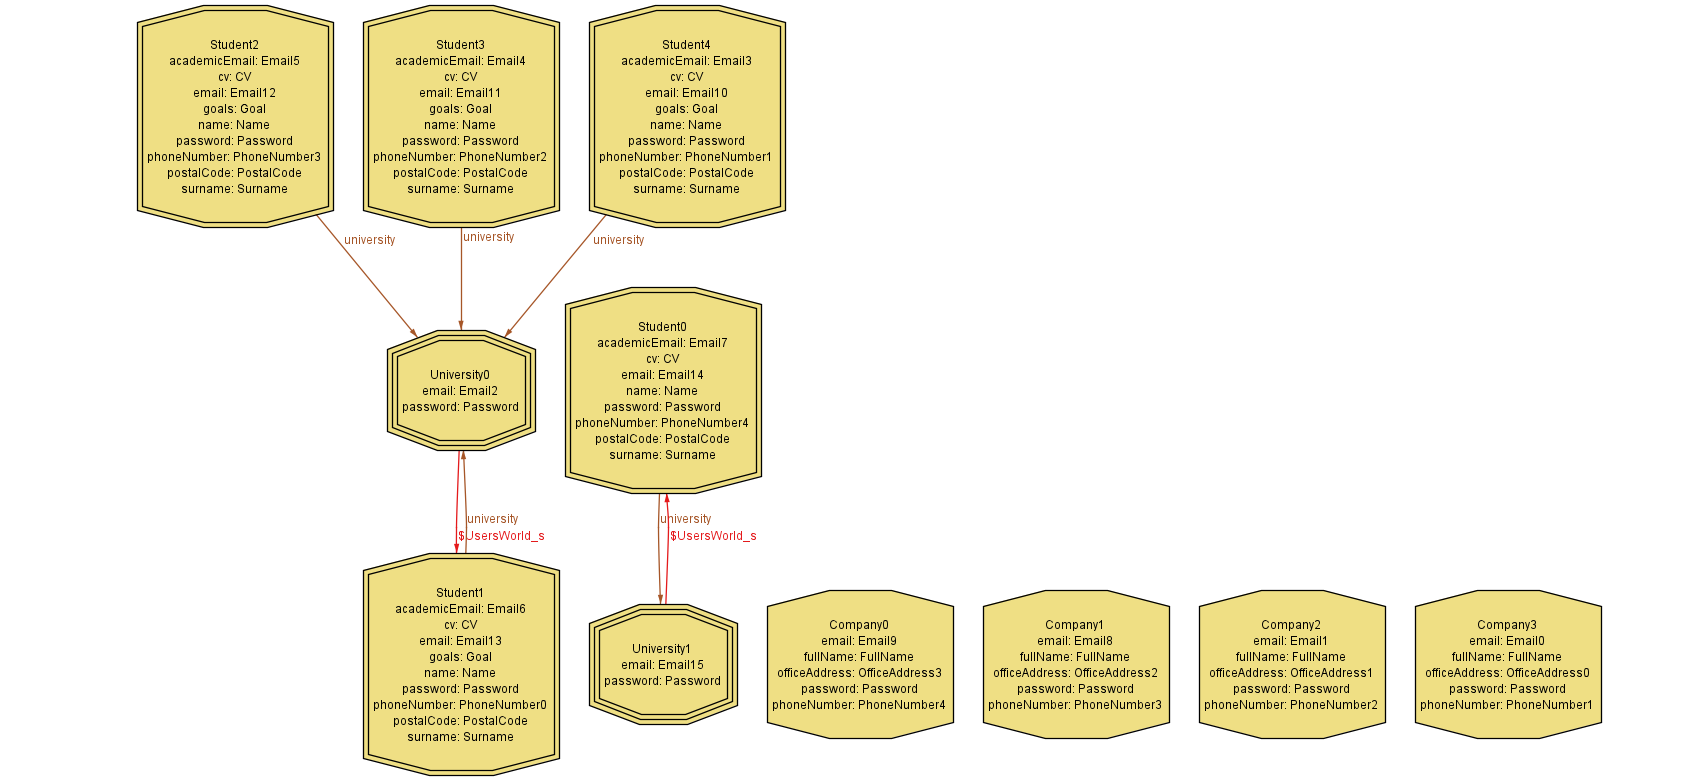
\includegraphics[width=0.5\linewidth]{Images/Alloy/Users.png}
    \caption{pred "UsersWorld" model}
    \label{fig:enter-label}
\end{figure}
\subsection{Internships and Internship offers}
This model describes the basic properties of the Internship and InternshipOffer entities.
\begin{figure}
    \centering
    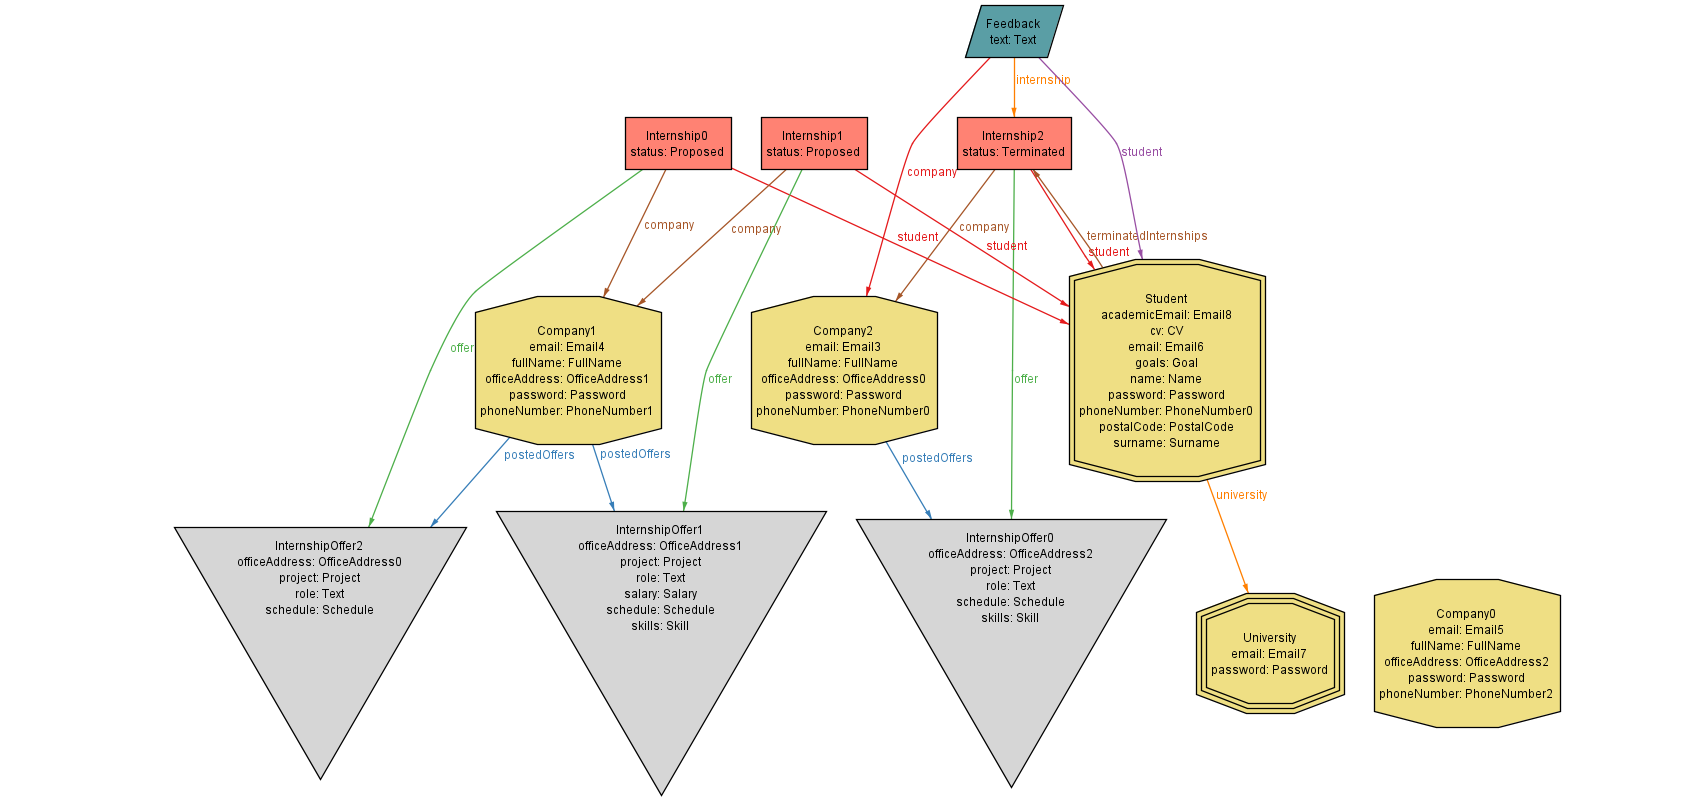
\includegraphics[width=0.5\linewidth]{Images/Alloy/Internship .png}
    \caption{pred "InternshipsWorld" model}
    \label{fig:enter-label}
\end{figure}
\subsection{Students applying to internships}
This model describes the interaction between Student, Internship and InternshipOffer when students start to apply to a specific offer. 
\begin{figure}
    \centering
    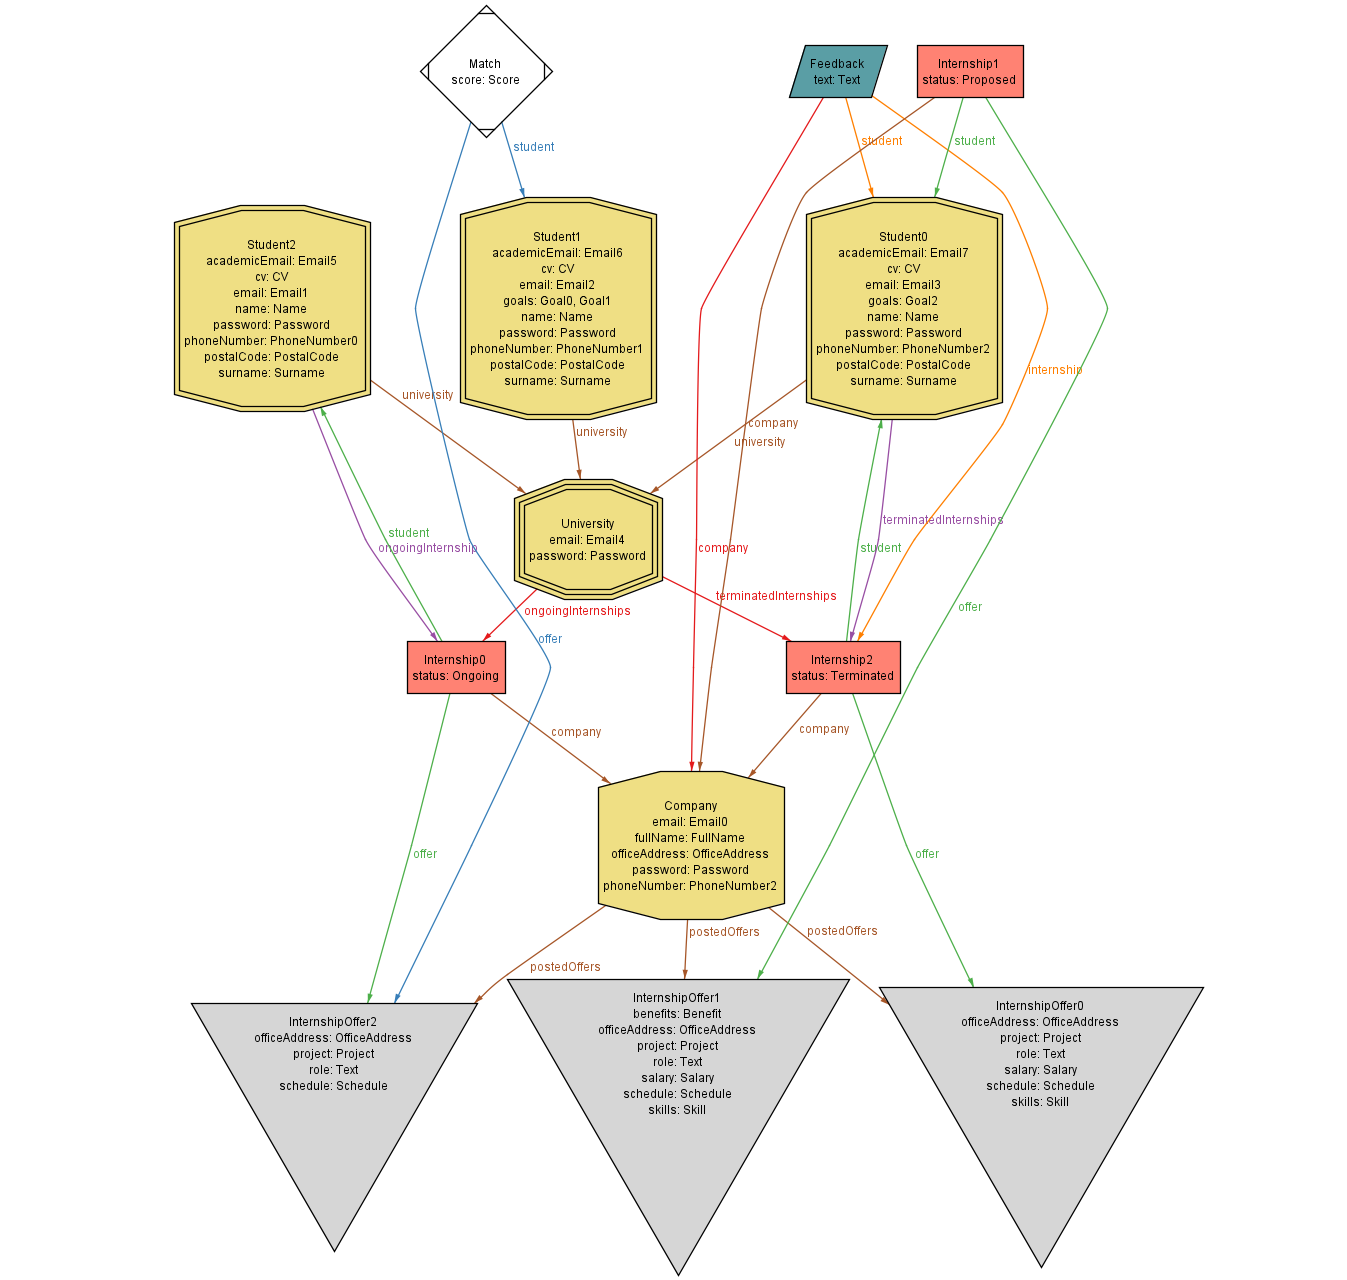
\includegraphics[width=0.5\linewidth]{Images/Alloy/Application.png}
    \caption{Pred "ApplicationWorld" model}
    \label{fig:enter-label}
\end{figure}
\subsection{Feedback and Complaint}
This model describes the relations between feedback and complaint entities and the other components of the system.
\begin{figure}
    \centering
    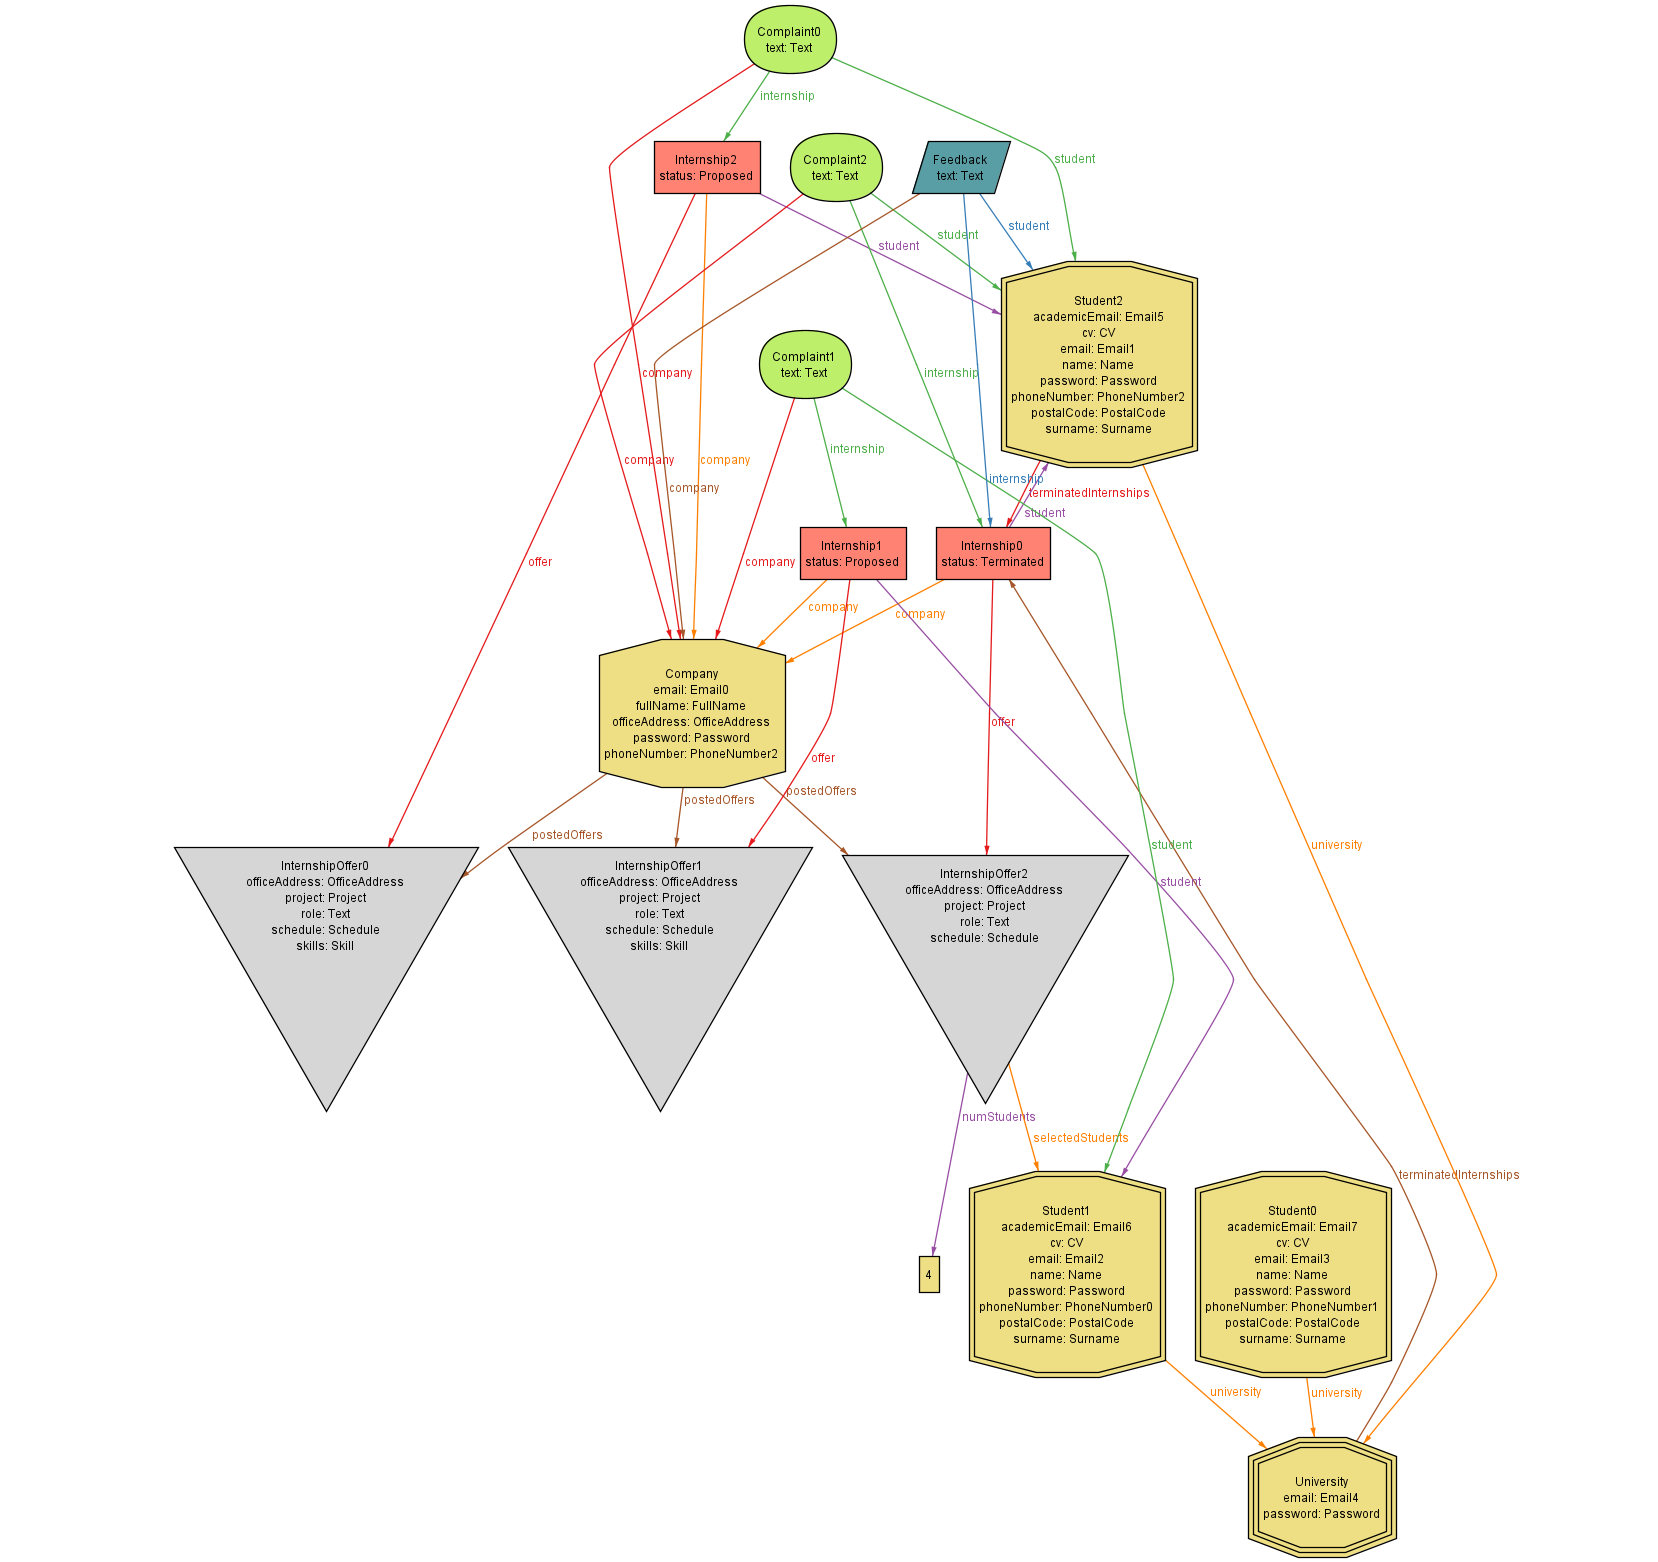
\includegraphics[width=0.5\linewidth]{Images/Alloy/ComplaintFeedback.png}
    \caption{Pred "FeedbackComplaintWorld" model}
    \label{fig:enter-label}
\end{figure}


    \chapter{Effort Spent}
    \label{ch:effort_spent}%
    \begin{table}[H]
    \begin{center}
        \begin{tabular}{c|c}
            \hline
            Member of group & Effort spent \\
            \hline
            Belfiore Mattia & \begin{tabular}{p{0.25\linewidth}|c}
                             Introduction          & $ 2h$\\
                             Overall description   & $7h$\\
                             Specific requirements & $13h$\\
                             Formal analysis       & $7h$\\
                             Reasoning             & $7h$\\
            \end{tabular} \\
            \hline
            Benedetti Gabriele & \begin{tabular}{p{0.25\linewidth}|c}
                             Introduction          & $5h$  \\
                             Overall description   & $2h$ \\
                             Specific requirements & $18h$ \\
                             Formal analysis       & $4h$\\
                             Reasoning             & $7h$ \\
            \end{tabular} \\
            \hline
            Buccheri Giuseppe & \begin{tabular}{p{0.25\linewidth}|c}
                                     Introduction          & $3h$ \\
                                     Overall description   & $5h$ \\
                                     Specific requirements & $18h$ \\
                                     Formal analysis       & $1h$ \\
                                     Reasoning             & $9h$ \\
            \end{tabular} \\
            \hline
        \end{tabular}
        \caption{Effort spent by each member of the group.}
        \label{tab:effor_spent}
    \end{center}
\end{table}



    \chapter{References}
    \label{ch:references}%
    \section{Paper references}
\label{sec:paper_references}%
\begin{itemize}
    \item \href{https://ieeexplore.ieee.org/document/8559686}{\textbf{ISO/IEC/IEEE 29148-2018}. Standard on requirement engineering.}
\end{itemize}


\section{Used tools}
\label{sec:used_tools}%
\begin{itemize}
    \item \href{https://github.com/MattiaBelfiore/BelfioreBenedettiBuccheri}{\textbf{GitHub}} for the project's version control.
    \item \textbf{AstahUML} for UML diagrams.
    \item \textbf{draw.io} for use case diagrams.
    \item \textbf{bpmn.io} for state diagrams.
    \item \textbf{Notion} for notes sharing.
    \item \textbf{OverLeaf} as collaborative online LaTex editor.
    \begin{itemize}
        \item PoliMi PhD Thesis Template on OverLeaf
    \end{itemize}
    \item \textbf{Alloy} for formal analysis.
\end{itemize}


% LIST OF FIGURES
    \listoffigures

% LIST OF TABLES
    \listoftables
    \cleardoublepage
\end{document}
